\documentclass{article}
\usepackage{setspace}
\usepackage{natbib}
\usepackage{amsmath}
\usepackage{float}
\usepackage{longtable}
\usepackage{booktabs}
\usepackage{lscape}
\usepackage{graphicx}
\usepackage{silence}
\usepackage{forest}
\usepackage{hyperref}
\usepackage{placeins}
\usepackage{textcomp} % Needed on Windows in Office
\usepackage{adjustbox}
\usepackage{xcolor}

\usepackage[toc,page]{appendix}


\let\Oldsubsection\subsection
\renewcommand{\subsection}{\FloatBarrier\Oldsubsection}

\newcommand{\comment}[1]{}

\author{Ann Atwater\footnote{Department of Economics, University of Florida.}}
\title{Understanding JetBlue's Anticompetitive Conduct \footnote{This is a preliminary draft. Please do not distribute without permission of the author. The author would like to thank the participants of the University of Florida Applied Microeconomics working group and of the Southern Economics Association 2024 conference for helpful feedback. Furthermore, the author would like to thank Brad Shrago for alerting her to important aspects of the ultra low-price carrier pricing strategy}}

\graphicspath{{05.Figures/}}

\AtBeginEnvironment{table}{\setlength\belowcaptionskip{-8pt}}

\begin{document}
	\maketitle
	
	\begin{abstract}
	This paper examines the counterfactual pricing effects of the world in which the proposed JetBlue-Spirit merger had been allowed to proceed. It finds evidence of modestly anti-consumer pricing effects. Beyond this, it also examines the concurrent Northeast Alliance's effects on pricing and network structures, finding limited evidence of pro-competitive pricing effects for airports in New York City and Boston. Finally, it provides evidence that consumer demand for air travel has become more elastic in the post-pandemic period, consistent with reporting of declines in business travel.


		\bigskip
		
	\noindent JEL Classification: L4, L41 \newline
	\noindent Keywords: airlines; mergers
		
	\end{abstract}
	
	\pagebreak
	
	\doublespacing
	
	\section{Introduction}
	\label{sec:Introduction}
	The 2020's saw the American aviation company JetBlue Airways involved with two different actions that would be found to be anticompetitive - the Northeast Alliance with American Airlines and an attempted merger with Spirit Airlines. The first of these saw it coordinating operations in four major airports within the northeastern United States, resulting in a state of affairs that was only slightly less than a merger with a competitor. The latter of these saw it attempting to purchase the nation's largest ultra-low cost carrier. 
	
	This paper's focus is on JetBlue's attempted merger with Spirit, and specifically the estimation of counterfactual pricing in the event that the merger would have been approved. However, estimation of this counterfactual is complicated by two factors. The first of these is the aforementioned Northeast Alliance. It began in 2020 and would be ultimately dissolved in 2023 following an adverse judgment in a lawsuit brought by the United States Department of Justice and Arizona, California, Florida, Massachusetts, Pennsylvania, Virginia, and the District of Columbia. As JetBlue attempted to acquire Spirit in 2022, while this alliance was still in effect, this complicates attempts to calculate counterfactual pricing due to American's role in shaping the route structure of JetBlue during this time, which would not have been present had the merger ultimately have been approved in 2023 or later. 
	
	Unfortunately, it is infeasible to simply use data from before the Northeast Alliance began due to the ramifications of the Covid-19 pandemic. This pandemic saw large changes to travel consumption within the United States, with business travel dramatically lower following the pandemic while consumer travel spending grew. This represents a structural change to the consumer base of the market in a way that makes direct extrapolation of the pre-pandemic period to the post-pandemic period difficult.
	
	To attempt to develop a full picture of the counterfactual world in which the merger was approved, I first analyze the impact of the Northeast Alliance on the overall operations and structure of JetBlue through a differences-in-differences approach. I find evidence for reductions in air fares of approximately 2\% at the airports focused on by the alliance, with these declines especially pronounced at Newark Liberty International Airport. However, as discussed in this paper, this may be partially by changes in the presence of JetBlue and American operations at airports outside of the four covered by the agreement due to supply constraints at the time of implementation, which could have increase the air fares at airports outside of the alliance beyond which would have occurred in the counterfactual world without the merger. 
	
	Following this, I estimate a structural demand model for both the pre- and post-pandemic periods. I observe that, in the counterfactual world in which the merger had been approved, one way fares would have been on average \$X higher in the post-pandemic markets and \$Y higher in the pre-pandemic markets. Air travel would have changed by {X} (X) and consumer surplus would have fallen by {Y} (Y) in the pre-pandemic (post-pandemic) periods. 

	With these findings outlined, the rest of the paper is organized as follows: Section \ref{sec:Literature} briefly summarizes the literature on airline mergers; Section \ref{sec:Setting} goes into detail on the American air travel market, the Northeast Alliance, and the JetBlue-Spirit merger; Section \ref{sec:Data} elaborates on my data sources; Section \ref{sec:Analysis} contains my analysis of the Northeast Alliance and the JetBlue-Spirit merger; finally, Section \ref{sec:Conclusion} summarizes the findings of this paper and examines their implications for antitrust policy going forwards. 
  
	\section{Literature Review}
	\label{sec:Literature}
	
	This paper analyzes the impact of JetBlue's conduct as it pertains to anticompetitive practices through an active alliance with American and through a court-blocked merger with Spirit. To accomplish this, it draws from the literature analyzing anticompetitive practices within the aviation industry and from the literature analyzing the impact of mergers within the aviation industry on consumer prices. Beyond this focus, it further develops our understanding of the role of low cost carriers and ultra-low cost carriers within the aviation industry through the analysis of more recent data.
	
	Since deregulation, and especially since the turn of the century, the aviation industry has seen a trend towards consolidation of existing carriers through mergers. Studies such as \citet{luo_price_2014} and \citet{carlton_are_2019} studying completed mergers of legacy airlines have generally found limited evidence of anticompetitive price effects in markets that both carriers were present in, generally attributed to the documented stronger competitive effects from low cost carrier presence within a market (such as in \citet{morrison_actual_2001, goolsbee_how_2008, shrago_spirit_2024}).\footnote{An alternative explanation suggested in \citet{le_market_2019} is that efficiencies from the Delta-Northwest and United-Continental mergers were sufficiently able to offset the upwards pricing pressure from increased concentration.} In contrast to these papers focused on mergers of legacy carriers, this paper focuses on a proposed (but ultimately uncompleted) merger between a low cost and an ultra-low cost carrier. As part of this analysis, it conducts a simulation of the merger of these two airlines. Recently, \citet{ciliberto_market_2021} and \citet{li_repositioning_2022} have used simulations of legacy carrier mergers to examine the implications of models which account for route entry decisions. Unlike these papers, I treat entry decisions as exogenous, owing in part to limitations from the post-pandemic changes to air travel demand.\footnote{A working paper, \citet{ewen_zoom_2023}, finds evidence consistent with a decline in business air travel of approximately two-thirds from 2019 to 2022.} 
	
	Beyond the literature on airline mergers, past research has examined anticompetitive practices within the aviation industry. \citet{miller_did_2010} examined the aftermath of a 1990's case against eight airlines involving potential collusion on fares through an electronic fare database used by travel agents. The author used an event study approach to determine that there was limited evidence of long term price effects from the court case. \citet{zou_assessing_2023} examined used differences-in-differences to examine the impact of the Northeast Alliance using data from its first year of operation. Unlike their paper, mine examines evidence from the entirety of the NEA through its unwinding in 2023. 
	
	Finally, my paper touches upon the literature examining the role of low cost and ultra-low cost carriers within the aviation industry. While this literature has predominantly focused on the ability of Southwest, the largest low cost carrier, on lowering prices within a market (e.g. \citet{windle_short_1995, morrison_actual_2001,  goolsbee_how_2008}), there has been movement in recent years to examine the effects of other low-cost carriers, such as JetBlue and Spirit, on prices. For example, \citet{shrago_spirit_2024} finds evidence that the presence of ultra-low cost carriers within a market increases the overall range of fares present within the market. My paper examines pricing effects of an ultimately unrealized merger between an ultra-low cost and low-cost carrier, allowing for an increased understanding of the differences between these two airline structures on competitive effects.  
	
	\section{Setting}
	\label{sec:Setting}
	
	Within this section, I establish key facts about the aviation industry in the United States in Subsection \ref{sec:Setting_Aviation}, then I discuss the Northeast Alliance and JetBlue-Spirit merger in more detail in Subsections \ref{sec:Setting_NEA} and \ref{sec:Setting_Merger} respectively.
	
	\subsection{United States Aviation}
	\label{sec:Setting_Aviation}
	The American airline industry is comprised of three major types of carriers: legacy carriers, low-cost carriers, and ultra-low cost carriers. Beyond their differences in pricing, the firms within each category operate differently. As such, it is worth spending time on these differences, as they inform later analyses within this paper.
	
	Legacy carriers are those firms that operated in the industry since before the 1978 deregulation of fares. At present, these are Delta, American, and United. The legacy carriers operate hub-and-spoke route networks which allow them to connect passengers from smaller markets through centralized hub airports to their final destinations. One consequence of this is that they operate a larger variety of aircraft within their fleets, allowing for more efficient flight operations to these smaller markets at the cost of additional crew training and maintenance expenditures.   
	
	The non-legacy air carriers are divided into two groups, the low cost and ultra-low cost carriers. Low cost carriers includes Southwest, Alaska,  Hawaiian, and JetBlue, while the ultra-low cost carriers are comprised of Spirit, Allegiant, and Frontier.\footnote{There exist a number of smaller, more regional focused low-cost carriers, such as Sun Country, which I do not refer to here. Later analyses within this paper treats products from these airlines as from a unified, "Minor Low-Cost Carrier" airline.} Unlike legacy carriers, both low cost and ultra-low cost carriers favor the usage of direct flights. While this requires them to eschew smaller markets, it allows them to avoid the costly expenditures relating to operating a hub airport. Furthermore, these carriers use only a handful of aircraft models within their fleets.\footnote{Figure \ref{fig:Fleet_Composition} graphs the average variety in aircraft models within each category of firm between 2007 and 2022.}

	Ultra-low cost carriers are distinguished from low-cost carriers through the practice of "unbundling," wherein ticket prices are lower but amenities traditionally included in a fare are additional purchases. While Ryanair in Europe had operated under this model since the early 1990s, a firm would not successfully adopt the strategy in the United States until Spirit introduced fees for checked baggage in April 2010 \citep{bachwich_emergence_2017}. While complaints regarding the quality of these airlines are well documented in consumer surveys and the press\footnote{For example in \citet{vasel_spirit_2016, elliott_jetblue_2022}.}, these airlines have managed a good deal of competitive success within their segment of the market. By the later part of the 2010s, trips on ultra-low cost carriers represented over a tenth of the total air travel within the United States (Figure \ref{fig:ULCC_Trips}).  Nonetheless, the industry is still dominated by the ``big four" carriers - the three legacy carriers and Southwest.  As depicted in Figure \ref{fig:BigFour_Ridership}, approximately 75\% of air travel in the United States is provided by these carriers. 
	
	 As documented in Figure \ref{fig:Spirit_fleet}, Spirit grew its fleet from under 50 planes before adopting the ultra-low cost model to nearly 200 planes by 2022. This expansion by Spirit brought it into increasing competition with JetBlue.\footnote{Historically, very few markets had multiple low cost carriers operating within them \citep{kwoka_fringe_2016, ciliberto_market_2021}. However, in recent years, there are approximately half as many markets with multiple low cost carriers operating within them as there are with a single carrier, as depicted in Figure \ref{fig:LCC_Count}.} As illustrated in Figures \ref{fig:JBSpirit_Airports_2012} and \ref{fig:JBSpirit_Airports_2022}, both firms primarily operate in airports situated along the east coast of the United States in addition to a few major cities in Texas and California, with Spirit's rapid expansion leading to both firms to increasingly operate out of the same airports.
	
	Despite these similarities in operations, both firms behaved differently in regards to competition by the 2020's.  In 2020, JetBlue created the ``Northeast Alliance" (NEA) with American Airlines, which saw them cooperate on setting flights originating to or departing from airports in New York and Boston.\footnote{Section \ref{sec:Setting_NEA} elaborates on this in more detail.} Beyond the NEA, the Department of Justice has alleged that JetBlue had taken part in anti-competitive behavior using the Airline Tariff Publishing Company to coordinate fares with other firms. 
	
	In contrast, Spirit would compete aggressively and became a maverick firm within the industry. It has maintained a consistent pace of increasing its fleet size over the course of the 2010s and into the 2020s (as graphed in Figure \ref{fig:Spirit_fleet}) despite the shock to air travel caused by the coronavirus pandemic.\footnote{As depicted in Figure \ref{fig:JetBlue_Fleet}, JetBlue's fleet stagnated following the pandemic due to it delaying orders for aircraft \citep{bellamy_iii_jetblue_2020, sipinski_jetblue_2020}.} This growth in its fleet was required for its consistent expansion into new air travel markets. As shown in \citet{shrago_spirit_2024}, this entry has resulted in greater competition than results from legacy carrier entry. In particular, markets entered by Spirit had increased variance in fares as existing carriers competed for the same highly cost concerned travelers that make up Spirit's core consumer base by offering paired back, "basic economy" products.
	
	Beyond the role of the firms within this industry, it is worth discussing the impact of the coronavirus pandemic on it as this shapes all analyses within this paper.  Between quarter 4 of 2019 and quarter 2 of 2020 saw a severe drop in air travel caused by a combination of fear of contracting the novel virus and the various regulatory closures of businesses leading to less incentive to travel. Air travel would recover to 2016 levels of air travel by approximately the second quarter of 2021 but would not recover to 2019 levels of air travel until halfway into 2022 (see Figure \ref{fig:QuarterlyPass}). 
	
	However, this recovery in ridership was not a full return to normal consumption patterns in airfare. Historically, business travel accounted for approximately a third of air travel (examples of these estimates can be found in \citet{berry_tracing_2010} or \citet{bet_market_2021}). However, following the pandemic, business travel reportedly decreased as businesses switched to telecommunications to meet, rather than traditional face-to-face meetings \citep{semuels_business_2021}. As such, consumption patterns are liable different, even if the levels are similar between the pre- and post-pandemic periods. 
	
	\subsection{Northeast Alliance}
	\label{sec:Setting_NEA}
	
	Prior to the attempted Spirit merger, JetBlue entered into the Northeast Alliance (NEA) with American Airlines. Finalized In January 2021, the NEA saw the two airlines coordinate operations in an attempt to act as if they were a single airline for any routes that touched upon the airports serving New York City and Boston. They jointly decided upon these routes, operate them so that consumers are indifferent between the two carriers for these routes\footnote{With the ultimate goal of keeping only one of the two firms active on a given segment, as per the ruling by Judge Leo Sorokin.}, and shared revenue between the firms earned from products within the agreement. The United States Department of Justice and the states of Arizona, California, Florida, Virginia, Massachusetts, Pennsylvania, and the District of Columbia brought a lawsuit against the agreement in September 2021 alleging that it violated the Sherman Antitrust Act.  Following a 2022 trial, the agreement would be found to violate the Sherman Antitrust Act in May 2023 and it was unwound in subsequent months\citep{rennison_jetblue-american_2023, rains_what_2023}.\footnote{Table \ref{tab:NEA_Timeline} details a timeline of key events relating to the NEA. Notably, some landing slot leases between the two airlines related to the merger experienced a gradual reversion to their original owners.} With this timeline outlined, I will now briefly discuss the features of the NEA and how it differed from traditional aviation alliances. 
	
	Alliances between aviation firms are commonplace within consumer aviation. For example, Delta is part of the ``SkyTeam Alliance" and United is part of the ``Star Alliance." These alliances see firms operating code sharing agreements between different carriers, in which airlines can seats on flights operated by other airline, with the ticket being under the ticketing airlines' code.\footnote{This allows, for example, for passengers of the Canadian airline Westjet to book connecting flights into the United States by using Delta flights for the domestic legs of their trip.}  These agreements are primarily operated between domestic carriers and international carriers to allow for better access to foreign markets by consumers. Benefits to consumers include the earning of frequent flier miles across all stages of a journey, regardless of the operating carrier, and easier handling of baggage. Meanwhile, carriers benefit from being able to offer a wider variety of destinations than would otherwise be possible using only routes that they themselves fly.
	
	Domestic aviation alliances are fairly rare. Two examples of them however include the NEA between JetBlue and American and the West Coast International Alliance (WCIA) between American and Alaska Airlines. Unlike alliances between domestic and foreign carriers, these agreements are generally unable to receive waivers from antitrust concerns through the Department of Justice. 
	
	Unlike normal alliances, the NEA was structured to act as if it was a merger between the two firms on affected routes. The two firms jointly scheduled flights within the selected cities, with the intent to minimizing overlap in routes offered, and coordinated on operations at the impacted airports.\footnote{One example of this coordination is the shuttle operated by the two airlines at JFK to allow customers to transfer between the terminals used by each airline without going through security a second time \citep{griff_riding_2021}.} Furthermore, as two of the impacted airports featured slot and gate controls,\footnote{A slot controlled airport is one in which airlines are assigned landing slots to allow for better coordination of runway usage in congested airports.} the NEA saw these firms share slot permits and coordinate on sharing gates at the effected airports. The ruling against the NEA found that this reduced the incentives of each firm to sell off owned slots or gates to other firms, increasing barriers to entry for companies wishing to serve the New York City market.
	
	As noted in the ruling by Judge Leo Sorokin, the existing alliance between Alaska and American called the WCIA serves as a direct contrast to how the NEA differed from traditional aviation alliances. Under the WCIA, fliers with one airline are able to book flights on the other. However, unlike under the NEA, routes covered by both carriers were excluded from codeshare bookings. Further differentiating it from the NEA, Alaska and American do not jointly determine scheduling nor capacity decisions across any markets. Nor do they share resources related to flight operations, such as landing and departure slots.\footnote{However, this should not be interpreted too strongly. Within the United States, only JFK, LGA, and DCA feature these restrictions. As such, this is less of a concern for the west coast focused alliance.} 
	
	 As documented in Table \ref{tab:NEA_Exposure}, approximately 75\% of JetBlue's routes, passengers, and revenue and 15\% of American's routes, passengers, and revenue were in the markets directly impacted by the four cities within the NEA. As such, the vast majority of JetBlue's fleet was deployed in collaboration with American. The ruling against the agreement indicated concerns that this coordination lessened JetBlue's ability to compete in even markets that were not coordinated within, due to the limited ability of JetBlue to increase its fleet size.\footnote{As noted in the judgment, there is limited ability to fully understand the ramifications of the NEA on JetBlue's route restructuring over this time period as it is coterminous with the changes within the industry caused by demand changes following the coronavirus pandemic.}
	
	\subsection{Attempted JetBlue-Spirit Merger}
	\label{sec:Setting_Merger}
	In February 2022, Spirit announced its intention to merge with fellow ultra-low cost carrier Frontier \citep{schaper_frontier-spirit_2022}. This prompted a counter offer from JetBlue in April for ownership of Spirit, which would lead to the attempted merger between Spirit and Frontier being called off in July amid a lack of support from Spirit shareholders \citep{josephs_jetblue_2022, josephs_spirit_2022}. By mid-October, Spirit shareholders approved the acquisition by JetBlue \citep{koenig_spirit_2022}. The next year would see the United States Department of Justice, the District of Columbia, Massachusetts, and New York file suit to block the merger in March \citep{chokshi_justice_2023}. Following a trial in the winter of 2023, the merger would be blocked on January 16, 2024, and the parties would ultimately decide against appealing the verdict \citep{chapman_jetblue_2024}.  These events are summarized in Table \ref{tab:JetBlue_Spirit_Timeline}. 
	
	JetBlue publicly considered the acquisition of Spirit to be a top priority for the company, choosing to not appeal the ruling blocking its Northeast Alliance with American Airlines in favor of focusing its resources on overcoming the lawsuit seeking to block the merger with Spirit \citep{aratani_jetblue_2023}. Beyond these legal resources, it directed resources towards trying to win public favor over the merger. Notably, it coordinated comment submissions to a Department of Transportation regulatory filing regarding the merger with pro-merger comments sourced from its employees.\footnote{Some employees went on to dispute that these comments accurately reflected their views see \citet{birnbaum_elizabeth_2023, birnbaum_jet-blue_2023} In Appendix \ref{sec:NaturalLanguage}, I use stance detection techniques to analyze comments left on this filing in more detail.} Despite this, following the ruling against the merger it would ultimately choose to drop its appeals, with some financial analysts noting a significant deterioration of Spirit's financial stability between 2022 and 2024 \citep{sider_jetblue_2024}. 
	
	I now turn my attention to the ruling by Judge Young which ultimately blocked the JetBlue-Spirit merger attempt. The judgment identifies five key cities for his ruling: Orlando, San Juan, Miami and Fort Lauderdale (termed "South Florida"), New York City, and Boston. These cities were identified on the basis that the majority of passengers in markets with competition between JetBlue and Spirit departed from these cities. These largely align with the cities in which the two firms would have the largest share of departing passengers within 2022 (Table \ref{tab:KeyCities}). However, the cities indicates ignores the firms' role in multiple smaller markets within Puerto Rico, namely Ponce and Aguadilla, where the two firms comprise the vast majority of the market. 
	
	In section 2.F of the judgment, the potential effects of the merger are listed as decreased airline seats, increased market concentration, increased debt for JetBlue, and increased prices for consumers. Table \ref{tab:JetBlueSpirit_Fleet} documents the aircraft in JetBlue and Spirit's fleets in 2022. Both airlines predominantly fly Airbus manufactured aircraft, with wider variety in JetBlue's fleet than Spirit's, using five different versions of the Airbus A321 aircraft\footnote{Two of these configurations reflect solely different seat configurations. The other three configurations are on the Airbus A321neo, a revision of the earlier aircraft.} Should Spirit's Airbus A320 and Airbus A321 were adjusted to the predominant seat configurations of JetBlue's aircraft, a total of 20 seats would be lost on each Airbus A320 and 69 seats would be lost on each Airbus A321, for a total of 4,799 seats lost. This would reflect a loss of approximately 13\% of the seats on Spirit's aircraft.\footnote{If instead, Spirit's Airbus A321 were adjusted to the 200 seat configuration rather than the 159 configuration, then this would be 3500 seats lost or a loss approximately 9.9\% of Spirit's seat capacity.} These rough calculations closely track the estimate of an 11\% reduction in seats accepted by the trial court in its decision.\footnote{The court further estimates a decline in annual departures of over 6.1 million. As I do not possess data on flight schedules, I am unable to assess this claim.} Beyond the issue of seats, this paper estimates the counterfactual increase in market concentration and increase in prices in Section \ref{sec:Analysis_NEA}. 

	\section{Data and Summary Statistics}
	\label{sec:Data}
	The primary dataset used in the creation of this paper is the Bureau of Transportation Statistics's Airline Origin and Destination Survey (DB1B) dataset. This is a 10\% sample of all domestic itineraries within the United States and includes data on pricing, length of air travel, carrier, and number of connecting flights. Within the literature, the DB1B has been the preferred data for domestic air travel for decades (e.g.  \citet{ciliberto_market_2021, berry_tracing_2010, goolsbee_how_2008, peters_evaluating_2006}). 
	
	 Within this industry, markets are defined by by origin airport, destination airport, year, and quarter. Within this definition, orinating and terminating airports are used as the determinants of a market rather than the metropolitan statistical areas that these airports reside in. This accounts for the known phenomenon that consumers do not treat airports within a metropolitan statistical area as interchangeable with each other.\footnote{For an example of this phenomenon, \citet{goolsbee_how_2008} observes differential impacts on pricing of prospective firm entry at the airport level than would be expected if airports were treated as interchangeable by consumers.} Within this paper, products within a market are further defined by carrier and non-stop status.\footnote{As such, each carrier is assumed to have either 0, 1, or 2 products within a market.} Appendix \ref{sec:DataProcessing} details the sample construction methodology and restrictions on markets within the sample (such as excluding markets that consist of airports that are fewer than 150 miles apart.)
	
	Market size is defined as the geographic mean of the population of the origin and destination metropolitan statistical areas population. This is a standard assumption within this literature (such as in \citep{ciliberto_market_2021}). This is calculated using the United State Census Bureau's annual estimates of metropolitan statistical area population. The outside good within a market is not consuming air travel between an origin and destination airport pair. As such, this includes instances where consumers choose to either not make a trip or to make the trip using an alternative method of transport, such as car or bus. 

    
	
	% In constructing my instruments for price, I used data on the spot price for jet fuel provided by the U.S. Energy Information Administration in addition to reported expenditures on jet fuel from airlines' P-12 filings with the Department of Transportation. The difference between the reported expenditures and the national average spot price is plotted in Figure \ref{fig:JetFuel}. The relative expenditures are fairly consistent for each airline, with the exception of Delta during the coronavirus pandemic and Southwest in 2022, with the latter deviation caused by fixed-price contracts filed in anticipation of an oil price shock due to the Russian invasion of Ukraine in 2022 \citep{mooney_southwest_2022}.  
	
	For the analysis of the Northeast Alliance in Section \ref{sec:Analysis_NEA}, data on state level coronavirus cases from the Centers for Disease Control and Prevention was used. Airport markets were assigned to this data on the basis of the state of the principal city within the origin and destination metropolitan areas.\footnote{For example, the New York City market was assigned New York}. State level data is used rather than county level data as this data is liable to be more accurate than county level data as coronavirus patients were able to test outside of their primary county. Furthermore, the virus saw seasonal trends that were regionally differentiated, suggesting that quarter level controls would be insufficient. Beyond this data, census bureau state-level and MSA-level estimates of personal income was collected for use in this analysis.\footnote{There is a significant delay in releases of these estimates for MSA. As such, the state-level data allows for a longer sample to be analyzed. On the shared quarters, I do not observe any notable differences in the estimated coefficients through the use of state or MSA level income data.}

    \begin{table}
    \caption{Product Level Summary Statistics}
    \label{tab:Summary_Statistics_Product}
    
\begin{tabular}[t]{llllll}
\toprule
 & Mean & (SD) & Minimum & Median & Maximum\\
\midrule
\addlinespace[0.3em]
\multicolumn{6}{l}{\textbf{Pre-Pandemic}}\\
\hspace{1em}Price (2017 USD) & 232.21 & ( 70.12 ) & 33.12 & 235.62 & 810.58\\
\hspace{1em}Passengers & 4248.33 & ( 10185.27 ) & 100 & 810 & 192050\\
\hspace{1em}Distance (1000s) & 1.41 & ( 0.67 ) & 0.15 & 1.28 & 3.87\\
\hspace{1em}Extra Distance & 0.13 & ( 0.18 ) & 0 & 0.06 & 1.66\\
\hspace{1em}Nonstop & 0.28 & ( 0.45 ) & 0 & 0 & 1\\
\hspace{1em}Origin Destinations & 29.97 & ( 33.37 ) & 1 & 13 & 180\\
\hspace{1em}Origin Prescence (\textbackslash{}\%) & 36.23 & ( 31.26 ) & 0.54 & 19.51 & 100\\
\hspace{1em}Delta & 0.25 & ( 0.43 ) & 0 & 0 & 1\\
\hspace{1em}American & 0.22 & ( 0.41 ) & 0 & 0 & \vphantom{1} 1\\
\hspace{1em}United & 0.14 & ( 0.35 ) & 0 & 0 & 1\\
\hspace{1em}Southwest & 0.25 & ( 0.43 ) & 0 & 0 & 1\\
\hspace{1em}JetBlue & 0.03 & ( 0.17 ) & 0 & 0 & 1\\
\hspace{1em}Spirit & 0.03 & ( 0.18 ) & 0 & 0 & 1\\
\hspace{1em}Other Carrier & 0 & ( 0.06 ) & 0 & 0 & 1\\
\hspace{1em}Observations & 307849 &  &  &  & \\
\addlinespace[0.3em]
\multicolumn{6}{l}{\textbf{Post-Pandemic}}\\
\hspace{1em}Price (2017 USD) & 212.77 & ( 75.21 ) & 27.96 & 209.94 & 737.78\\
\hspace{1em}Passengers & 3531.43 & ( 8648.27 ) & 100 & 690 & 144930\\
\hspace{1em}Distance (1000s) & 1.41 & ( 0.67 ) & 0.15 & 1.28 & 3.86\\
\hspace{1em}Extra Distance & 0.14 & ( 0.19 ) & 0 & 0.07 & 1.83\\
\hspace{1em}Nonstop & 0.26 & ( 0.44 ) & 0 & 0 & 1\\
\hspace{1em}Origin Destinations & 29.24 & ( 33.72 ) & 1 & 12 & 187\\
\hspace{1em}Origin Prescence (\textbackslash{}\%) & 34.77 & ( 30.92 ) & 0.53 & 18.42 & 100\\
\hspace{1em}Delta & 0.22 & ( 0.41 ) & 0 & 0 & 1\\
\hspace{1em}American & 0.22 & ( 0.41 ) & 0 & 0 & 1\\
\hspace{1em}United & 0.13 & ( 0.34 ) & 0 & 0 & 1\\
\hspace{1em}Southwest & 0.26 & ( 0.44 ) & 0 & 0 & 1\\
\hspace{1em}JetBlue & 0.03 & ( 0.16 ) & 0 & 0 & 1\\
\hspace{1em}Spirit & 0.04 & ( 0.2 ) & 0 & 0 & 1\\
\hspace{1em}Other Carrier & 0.01 & ( 0.1 ) & 0 & 0 & 1\\
\hspace{1em}Observations & 265196 &  &  &  & \\
\bottomrule
\end{tabular}

    \footnotesize{A product is defined as a set of origin airport, destination airport, year, quarter, firm, and nonstop status. "Origin Destinations" is the number of airports served from the originating airport across all firms, "Origin Prescence" is the fraction of these destinations served by the ticketing carrier. The pre-pandemic sample includes all quarters of the years 2017 through 2019. The post-pandemic sample includes data from the second quarter of 2021 through the second quarter of 2023.}
    \end{table}

    Summary statistics for product level data are included in Table \ref{tab:Summary_Statistics_Product}. Roughly three-percent of the products included in the final sample belong to each of JetBlue and Spirit, consistent with their smaller network sizes than the legacy carriers and Southwest. There is a slight, roughly \$20 decrease in airfare following the pandemic, however, this is not statistically distinct from the fares in the pre-pandemic period. Product characteristics relating to network structure, such as travel distance and nonstop status and also unchanged between the two periods, consistent with the idea that the observed changes in the customer base between these two periods did not result in firms substantially changing their offerings.  

    Summary statistics for market level characteristics are included in Table \ref{tab:Summary_Statistics_Market}

    \begin{table}
        \caption{Market Level Summary Statistics}
        \label{tab:Summary_Statistics_Market}
        
\begin{tabular}[t]{llllll}
\toprule
 & Mean & (SD) & Minimum & Median & Maximum\\
\midrule
\addlinespace[0.3em]
\multicolumn{6}{l}{\textbf{Pre-Pandemic}}\\
\hspace{1em}Minimum Miles (1000s) & 1.18 & (0.64) & 0.15 & 1.02 & 2.95\\
\hspace{1em}Average Miles (1000s) & 1.23 & (0.66) & 0.15 & 1.07 & 3.02\\
\hspace{1em}Number of Firms & 2.94 & (1.49) & 1 & 3 & 9\\
\hspace{1em}Number of Products & 3.52 & (2.11) & 1 & 3 & 15\\
\hspace{1em}Number of Customers & 14970.24 & (28280.06) & 260 & 4150 & 406050\\
\hspace{1em}HHI & 8017.21 & (4297.27) & 1611.61 & 7043.02 & 20000\\
\midrule
\hspace{1em}Observations & 87363 &  & JetBlue Markets & 7442 & \\
\hspace{1em}JetBlue \& Spirit Markets & 1533 &  & Spirit Markets & 7474 & \\
\midrule
\addlinespace[0.3em]
\multicolumn{6}{l}{\textbf{Post-Pandemic}}\\
\hspace{1em}Minimum Miles (1000s) & 1.19 & (0.64) & 0.15 & 1.04 & 2.96\\
\hspace{1em}Average Miles (1000s) & 1.24 & (0.66) & 0.15 & 1.1 & 2.98\\
\hspace{1em}Number of Firms & 3.21 & (1.56) & 1 & 3 & 9\\
\hspace{1em}Number of Products & 3.79 & (2.16) & 1 & 3 & 14\\
\hspace{1em}Number of Customers & 13375.81 & (25085.61) & 230 & 3840 & 317370\\
\hspace{1em}HHI & 7479.76 & (4410.86) & 1460.46 & 6260.03 & 20000\\
\midrule
\hspace{1em}Observations & 70016 &  & JetBlue Markets & 5945 & \\
\hspace{1em}JetBlue \& Spirit Markets & 1554 &  & Spirit Markets & 9123 & \\
\bottomrule
\end{tabular}

        \footnotesize{A market is defined as a set of origin airport, destination airport, year, and quarter. The average miles reported within a market is weighted by itinerary passengers. The pre-pandemic sample includes all quarters of the years 2017 through 2019. The post-pandemic sample includes data from the second quarter of 2021 through the second quarter of 2023. }
    \end{table}

	\section{Analysis}
	\label{sec:Analysis}
	
	This section is organized into four subsections. In Section \ref{sec:Analysis_NEA}, I use a synthetic control design to analyze the Northeast Alliance's effects on airfare. Following this, I compare the results from this with the differences-in-differences estimation results common from the literature and examine the ramifications of the alliance for simulating the counterfactual world in which the JetBlue-Spirit merger was allowed to occur. In Section \ref{sec:Analysis_Demand}, I develop a structural model of demand for the airline industry and analyze its results. In Section \ref{sec:Analysis_Supply}, I develop the structural model of supply for the airline industry used in conjunction with the demand model for the counterfactual merger simulation detailed in Section \ref{sec:Analysis_Merger}. 
	
	\subsection{Northeast Alliance}
	\label{sec:Analysis_NEA}

    
        
	The first of these areas of investigation is to evaluate the NEA's impact on itineraries where passengers take flights operated by both JetBlue and American within a single, unidirectional trip. Empirically, it is clear that the number of interline itineraries featuring travel provided by both providers increased following the implementation of the NEA (see Figures \ref{fig:NEA_Mix_AAB6} and \ref{fig:NEA_Mix_B6AA} for the number of tickets). 
	
	To analyze this, for origin-destination airport pair $j$ at time $t$,  I estimate the model \[Y_{jt} = \alpha N_{j} + \sum_{T = -8}^{8} \delta_{T} P_{t = T} + \sum_{T = -8, t = 8}^{8} \gamma_{T} N_{j} P_{t = T} + \epsilon_{jt}\] where $Y_{jt}$ is a dummy variable that is 1 if at least one itinerary was recorded that featured flights by both JetBlue and American,  $N_{j}$ is a dummy variable if at least one endpoint airport was covered by the NEA agreement, $P_{t = T}$ is a variable which is 1 if $t = T$ and 0 otherwise, and $\epsilon_{jt}$ is a random error term.\footnote{Minimal controls are used in this regression as the NEA agreement is the core determinant of codesharing itineraries between JetBlue and American. As such, any codesharing itineraries will be necessarily caused by this agreement.} In defining periods in this, and later analyses within this section, I define 2019 quarter 4 as period "-1", and 2021 quarter 2 as period "0". This excludes the entire duration of the pandemic before widespread vaccine availability.\footnote{As depicted in Figure \ref{fig:QuarterlyPass}, the second period of 2021 saw air travel return to 2016 levels. As such, this should represent a more typical environment for the industry.} Results for this estimation are included in Table \ref{tab:NEA_Switch_Prob} and the coefficients are plotted in Figure \ref{fig:NEA_Joint_Op}. As would be expected, negligible codesharing itineraries are booked before the start of the NEA, following which the probability that a market impacted by the agreement would include these itineraries rose to approximately five to seven percentage points. 
	
	Beyond the numerical significance of these estimates, these results suggest a timeline for when the agreement was most implemented, namely the fourth quarter of 2021.\footnote{This is period 2.} This is despite the NEA beginning to accept codesharing bookings in February of 2021 on 80 routes \citep{griff_8_2021}. As such, this is consistent with the concern that past research might understate the effects of the NEA as the period observed was limited to the first four quarters of operation.
	
	 I turn my attention to identifying its effects on air fare. Past literature in the aviation industry has used one of two outcomes of interest: either the average market fare or the average per-mile fare (which is called the market yield.  While the literature has largely focused on fares in evaluating the effects of anticompetitive practices and mergers within retrospective studies (such as in \citet{luo_price_2014, carlton_are_2019}), the only existing study \citep{zou_assessing_2023} to evaluate the NEA focused on yields as its variable of interest. As such, my estimations are conducted on both fares and yields to allow for comparison with both strands of literature. 
	
	 I now turn my attention to the difference in average fares within markets with itineraries listing both airlines as the ticketing carrier.  I model the difference between the average American and average JetBlue fares $Y_{jt}$ for market $j$ in period $t$ as \[Y_{jt} = \alpha N_{j} + \sum_{T = -8}^{8} \delta_{T} P_{t = T} + \sum_{T = -8, t = 8} \gamma_{T} N_{j} P_{t = T} + \beta X_{jt} + \epsilon_{jt}\] where $N_{j}$ is a dummy variable if the market includes an endpoint covered by the NEA agreement, $P_{t = T}$ is a variable which is 1 if $t = T$ and 0 otherwise, $X_{jt}$ is a vector of additional market level controls which includes the log of the geometric mean income of the origin and destination metropolitan statistical areas, the log of the geometric mean population of the origin and destination metropolitan statistical areas, the lagged HHI for these markets, state coronavirus rates, and the share of flights within each market that are direct. Finally, $\epsilon_{jt}$ is a random error term. 
	 
	 The results for this estimation are contained in Table \ref{tab:NEA_Fare_Neutral} and graphed in Figure \ref{fig:NEA_Fare_Neutral}.\footnote{ Results for the average market yield are included in Table \ref{tab:NEA_Yield_Neutral} and Figure \ref{fig:NEA_Yield_Neutral} and follow the same trend.} I estimate that after the third quarter of the NEA's operation, this difference was consistently lower by about \$75 dollars within markets impacted by the NEA. This decline is consistent with the collaborating firms' stated desire for consumers to treat products offered by each firm as neutral and the timeline is consistent with my results in Table \ref{tab:NEA_Switch_Prob}. I fail to observe evidence of pretrends, lending credence to the argument that the NEA reduced the price spread between American and JetBlue tickets. However, this result does not clarify if this was caused by American fares becoming less expensive or JetBlue fares becoming more expensive. 
	
	Finally, I estimate the average fare within market $j$ at time $t$ using the prior model, but with $Y_{jt}$ now being this average fare across all airlines.  These results are included in Table \ref{tab:NEA_Market_Fare} and the event study coefficients are plotted in Figure \ref{fig:NEA_Market_Fare}.\footnote{The corresponding yield table and graph are Table \ref{tab:NEA_Market_Yield} and Figure \ref{fig:NEA_Market_Yield} respectively} While these coefficients are statistically significant and negative outside of the first two periods of the NEA, it is difficult to draw a conclusion that this is an effect of the NEA as it aligns with average fares in most of the pre-periods. 
	
	To understand possible heterogeneity between airports, I then estimated an alternate specification where the variable for NEA membership is instead replaced by a set of four variables, one for each airport covered by the agreement. These results are plotted in Figure \ref{fig:NEA_Airport_Fare_Interaction}. While the results for both JFK and LGA in New York City exhibit the same pattern above, the fares at EWR are consistently lower than fares within the pre-period, suggesting that the NEA had reduced fares at this airport. By contrast, the fares at BOS. are consistently higher than the pre-period fares, suggesting that the NEA increased fares for Boston markets.
	
	 That the coefficients for Newark are negative is consistent with the evidence from Table \ref{tab:NEA_Airport_Prescence} that markets with Newark as the originating airport had the least overlap between the carriers before the agreement, suggesting that possible anticompetitive effects from the merger were limited for these markets. 
	
		These results support the findings of \citet{zou_assessing_2023}. 
	

	
	\subsection{Spirit Merger}
	With these findings regarding the Northeast Alliance established, I now turn my attention towards estimating the effect that the JetBlue-Spirit merger would have had on prices had it been allowed to be completed. To do this, I estimate a model of demand, assume that Bertrand-Nash competition with differentiated products describes the supply side of the market, and then estimate three merger counterfactuals wherein the resulting merged firm would have inherited the least, average, and greatest marginal cost for the resulting post-merger products of the individual firms. 
	
	Before beginning these analyses, it is important to consider the implications of one critical assumption used within them, namely that firms treat overall market structure as exogenously determined. The largest consequence of these is that routing cannot respond to demand shocks within a given quarter. Furthermore, this assumption does not allow for the merging firms to change which markets they operate in following the merger.
	
	This creates a problem for proper inference of the counterfactual world in which the merger had been completed. As determined in the previous subsection, the NEA had included a reorganization of the route networks of each of the collaborating firms as part of the agreement. As such, counterfactuals using markets between 2021 and 2023 are those in which the JetBlue-Spirit merger is allowed to be completed while the NEA is in effect and without any resulting reorganization of routes. 
	
	Unfortunately, it is not possible to simply use markets from before the implementation of the NEA as this would require the usage of data from either during the worst of the decline in air travel caused by covid-19 or before it. As documented in press sources and in a working paper \citep{ewen_zoom_2023}, air travel demand dynamics have greatly changed following the pandemic. In part thanks to the rise of telecommunications software such as Zoom, low-price elasticity business travel has lessened. Furthermore, as consumers were able to increase savings during the pandemic period (CITATION NEEDED), they are liable to have become less price sensitive following the resumption of mass tourism. 
	
 	To try to resolve these issues, I conduct all analyses within this section on two samples - the "pre-pandemic" sample from the first quarter of 2017 through the fourth quarter of  2019 and a "post-pandemic" sample consisting of data from the third quarter of 2021 through the end of the second quarter of 2023. By comparing the results from these two samples, a more complete picture can emerge of the counterfactual world in which the JetBlue-Spirit merger had been completed despite the issues facing each sample's overall credibility.  
 	 	 
 	 % Route Dynamics
 	 %	The Northeast Alliance between JetBlue and American poses an issue for proper counterfactual merger simulation between JetBlue and Spirit for two key reasons. The first of these is that the alliance saw the reorganization of JetBlue and American's route networks to allow them to compete more effectively against Delta and United within the New York and Boston markets. As my estimation of demand in Section \ref{sec:Analysis_Demand} treats network decisions as exogenous, this impedes proper counterfactual estimation.  The second is that through the codesharing agreement, each of these firms has products within my dataset that were not able to be fully offered by the firm alone.\footnote{This is further exacerbated by the restructuring of each firm's operations between these airports to have each route specialize on some routes.} In summation, there are observed products which would not have been offered absent the alliance while there are unobserved products which would have been offered absent the alliance. 
 	 
 	 %	Gaining an understanding of the breadth of the reorganization of the two airlines routes is difficult, but a helpful clue is present within the ruling against the agreement. The ruling notes that a goal of the reorganization in routes was to ensure that either JetBlue or American, but not both, were present in a given route between two cities. This suggests that understanding of the reorganization can be gained by estimating $P(AA \in R \mid JB \in R)$ and $P(JB \in R \mid AA \in R)$ as functions of a route being an "NEA Route" (that is, a route that touches on an airport in the New York City or Boston markets), distance and time.\footnote{Unlike in most other analysis of this paper, here we are interested in which airline is operating the planes on a given route, and so products are assigned to the operating carrier rather than the ticketing carrier.} These results are reported in Table \ref{tab:NEA_Op_Prob}.
 	 
 	 %	The observed products problem is easier to gain an understanding of. Figures \ref{fig:NEA_Mix_AAB6} and \ref{fig:NEA_Mix_B6AA} plot the number of estimated passengers on itineraries with American or JetBlue listed as the ticketed carrier and at least one leg of the journey on a flight operated by the other carrier. Two facts are apparent from this graph - the first is that despite the NEA agreement having been finalized in the first quarter of 2021, it took a good deal of time for JetBlue and American to allow their customers to book using the cross sharing provisions. The second is that from the first quarter of 2022 to the dissolution of the agreement in the third quarter of 2023, roughly 500,000 passengers would fly on itineraries made possible by the agreement. This accounts for roughly 5\% of the airlines' passengers for these NEA routes within this period. 
 	 	 
	\subsubsection{Demand Model and Results}
	\label{sec:Analysis_Demand}
	I use a random coefficient nested logit model to estimate demand, in line with the model originally documented in \citet{berry_automobile_1995}. Adopting the best notation described in \citet{conlon_best_2020}, each consumer $i$ in market $t$ has indirect utility from buying product $j$ as defined by 
	
	\[U_{ijt} = \delta_{jt} + \mu_{ijt} + \epsilon_{ijt}\]
	
	Where $\delta_{jt}$ is the mean utility across consumers in market $t$ for product $j$, $\mu_{ijt}$ is consumer level deviation from this mean utility, and $\epsilon_{ijt}$ is an unobserved consumer-level shock. $\delta_{jt}$ is parameterized as \[\delta_{jt} = \alpha p_{jt} + x_{j} \beta + F_{jt}\gamma  +  \epsilon_{jt}\] where $p_{jt}$ is the price of product $j$ in market $t$, $x_{jt}$ is a vector of observed itinerary characteristics\footnote{Namely nonstop status and miles flown}, and $\epsilon_{jt}$ is a product level shock shared by all consumers within a market. Within this model, $\mu_{ijt}$ is parameterized as \[\mu_{ijt} = \sigma_{p} p_{jt} \nu_{ip} + \sum_{k} \sigma_{k} x_{kjt} \nu_{ik} \] with the $\nu$ parameters drawn from a  normal distribution with mean zero and estimated variance. Finally, $\epsilon_{ijt}$ are assumed to arise from a type 1 extreme value distribution so that market shares will be of the discrete choice nested logit variety. Within this model specification, air fare is included within one nest while the outside good is included in the other nest.
	
	Consumer $i$ purchases itinerary $j$ if it has greater utility than all other products in the market. As such, market shares can be obtained by integrating over the consumers, resulting in the market share of each product defined by \[s_{jt} = \int \frac{e^{\delta_{jt} + \mu_{ijt}}}{\sum_{j'} e^{\delta_{jt} + \mu_{ijt}}} d{\nu_{i}}\]
	
	Within this model, the contribution to utility shared by consumers, $x_{jt}$, contains the distance between the origin and destination airports within the market, the squared distance, a dummy variable which is one if an itinerary does not include any intermediate stops between the origin and destination airports, the difference between the miles flown by the itenary and the minimum number of miles flown within the market, the square of this difference, a dummy variable which is 1 if the origin or destination airport are in Florida or Las Vegas, and the ratio of the number of destinations served out of the origin airport by the carrier divided by the total number of destinations served out of that airport. This last measure is intended to proxy for rewards program strength of the carrier at the origin airport. $F_{jt}$ is a vector of controls which includes fixed effects for each year-quarter and carrier. The variables included in $x_{jt}$ are intended to be largely unresponsive to demand shocks - these characteristics of a product are determined primarily by a carrier's route structure and the geography between the origin and destination airports. 
	
	 Four sets of instruments are used to account for the endogeneity of prices and shares within a market. The first set consists of cost shifters created by multiplying dummy variables for origin or destination airport being a hub of the ticketing carrier by the miles traveled and the square of the miles traveled. The second set of instruments, employed to account for endogeneity in market shares, consists of the differentiation instruments described in \citet{gandhi_measuring_2019} constructed from a dummy variable that is 1 for a nonstop flight, the miles covered by the itinerary, the square of the miles covered by the itinerary, and the service ratio of the carrier out of the destination airport. The third set of instruments, employed to instrument for the nesting parameter $\lambda$ consists solely of the number of products within a market. Finally, all remaining exogenous regressors and their interactions comprise the final set of instruments.\footnote{Other instruments for price were considered, including interactions between the gas miles variable and characteristics of the origin airport and interactions between the exogenous variables. However, the selection of price shifters used in the final model had the best performance across the tests documented in Tables \ref{tab:Instrument_Compare_Pre}. The final specification chosen (column 4) has the benefit of passing the Wu-Hausman test while failing the Test of Over Identification by the least amount of the tested models. As noted in \citet{nevo_measuring_2001}, provided enough observations it is virtually impossible to pass the over-identification test, and as such, I am not concerned with the result. For comparison purposes, the instrument comparison table on the main period of interest (2021 Q2 through 2023 Q2) is included as Table \ref{tab:Instrument_Compare}.}
	
    Results for the estimation of this model's coefficients are included in Table \ref{tab:DemandEst}.

    \begin{table}
        \caption{Demand Estimation Results}
        \label{tab:DemandEst}
        
\begin{tabular}[t]{lll}
\toprule
Variable & Post-Pandemic & Pre-Pandemic\\
\midrule
Price & -3.114 & -2.947\\
 & (0.44) & (0.34)\\
\midrule
Price & 0.599 & 0.59\\
 & (0.12) & (0.12)\\
\midrule
Nesting Parameter & 0.115 & 0.136\\
\addlinespace
 & (0.032) & (0.045)\\
\midrule
Period & 2017Q1-2019Q4 & 2021Q2-2023Q2\\
N Products & 265196 & 307849\\
N Markets & 70016 & 87363\\
Mean Elasticity & -5.211 & -5.323\\
\addlinespace
Spirit Mean Elasticity & -3.44 & -3.15\\
JetBlue Mean Elasticity & -5.18 & -5.16\\
Mean Markup & 0.21 & 0.203\\
\bottomrule
\end{tabular}

        \footnotesize{$^{***}p<0.01$; $^{**}p<0.05$; $^{*}p<0.1$ Products are defined as a Carrier-Nonstop pair within an Origin-Destination-Year-Quarter market. Origin Service Ratio is the fraction of direct routes out of the originating airport operated by the carrier divided by the number of distinct direct routes out fo that airport. Extra Miles is the average additional miles flown with a connecting itinerary minus the minimum miles flown within a market.  A tourist product is one that serves the Las Vegas metropolitan statistical area or an airport in Florida.}
    \end{table}
	
	% Finally, I estimate the mean price elasticity of demand in both periods as well as the mean price elasticity of demand for products offered by JetBlue and Spirit in both periods. I estimate that the mean own-price elasticity across all products is approximately -4.73 in the pre-pandemic period and approximately -5.946 in the post-pandemic period. This is consistent with an observed decline in business travel following the pandemic as firms became used to telecommunications software such as Zoom for business meetings. As business travelers are less price sensitive than leisure travelers, it is reasonable for such a change in price elasticity to occur in such a limited time. Furthermore, the pre-pandemic price elasticity is consistent with past estimates of price elasticity, as detailed in Table \ref{tab:ElasticityComparison}.
	
	Similarly to the overall change in estimated price elasticity following the pandemic, the products of both JetBlue and Spirit became more elastic following the pandemic. However, in both periods, Spirit's products are more price-inelastic than those of JetBlue, consistent with its status as the often lowest cost carrier in the market, serving as an alternate to higher priced air fares.  
	
	\subsubsection{Supply Model and Results}
	\label{sec:Analysis_Supply}
	The consumer aviation market is assumed to operate under Bertrand competition with differentiated products following the exogenous determination of quarterly route structure. This allows for recovery of marginal costs through the estimated demand elasticities.  These are included with the estimates of Demand within Table \ref{tab:DemandEst}. I estimate a decline in observed markups of approximately X percentage points between the pre- and post-pandemic periods. 
	
	
	\subsubsection{Merger Simulation}
	\label{sec:Analysis_Merger}
	I can now turn my attention to simulation of the Spirit-JetBlue merger. For each of the pre-pandemic and post-pandemic periods, I estimate four counterfactuals: one which represents the scenario in which product characteristics remain unchanged following the merger (a "basic" simulation) and three in which various levels of efficiencies are realized following the merger (the "best case", "average case", and "worst case" simulations).
	
	 Should the merger have been approved, there would have been a period of time in which JetBlue would be operating the Spirit fleet largely as is, due to factors such as the time needed to renovate aircraft from the Spirit seating configuration to the JetBlue configuration and legal delays relating to the change in ownership of permits. As such, the basic simulation provides an insight into the "short-run" pricing impacts resulting from the merger. Furthermore, in this time period, the key possible pricing effects are reflected in JetBlue's ability to internalize the price externalities from the Spirit products. As Spirit had a reputation as a maverick firm, these are able to be significant to consumer welfare, even if they make up a distinct minority of tickets in the market.
	 
	 Tables \ref{tab:Simulation_Pre_Basic} and \ref{tab:Simulation_Post_Basic} contain the results from this simulation. As would be expected, 
	
	With the First, using the demand estimates and the assumptions on firm conduct described above, I estimate the marginal cost of each product. Following this, I reconstruct the product data by assigning all Spirit itineraries to JetBlue, and then assuming that the combined firm's connecting products will take on the more efficient routing available, reducing the average miles flown to the lower of the two firm's within a given market. Following this, I assign these merged products the lowest, average, and greater of the marginal costs of the original products, creating three separate data sets for the examination of different levels of efficiencies resulting from the merger. These scenarios are, respectively, the best-case, average-case, and worst-case scenarios for the post-merger firm's cost structure.  
	
	The results for these counterfactual estimations on the markets in which both firms operated in are reported in Table \ref{tab:Simulation_Post} for the post-pandemic period and in Table \ref{tab:Simulation_Pre} for the pre-pandemic period. 
	
	%The first of these is the "Separate Product" counterfactual in which the Spirit brand continues to exist. This scenario can be thought of as representing the time period during which Spirit's brand would exist following the merger but which JetBlue could internalize the price-externalities of Spirit products during.\footnote{This time period is liable to be significant. Within the trial regarding the merger, JetBlue's lawyers indicated that it would take until 2025 to start changing the seat configurations on the acquired Spirit aircraft. This sort of delay is common with airline mergers. For comparison, the United-Continental merger took over eighteen months to combine operations once it was approved.}
	
	%	[In next version - will estimate the effect of Spirit being removed from markets and replaced by JetBlue in markets both firms did not operate in. Want to capture maverick removal.]

	
	\section{Conclusions}
	\label{sec:Conclusion}
	
	\pagebreak 
	\bibliography{airline} 
	\bibliographystyle{abbrvnat.bst}
	\FloatBarrier
	
\pagebreak	\begin{appendices}
	
	\section{Data Processing Methodology}
	\label{sec:DataProcessing}
	As detailed in Section \ref{sec:Data},	the Bureau of Transportation Statistics's Airline Origin and Destination Survey (DB1B) database was the primary data set used for this research. After compiling the DB1B into a single dataset for the years 2015 through the second quarter of 2023, some observations were excluded from the sample. Itineraries with fares lower than \$15 were excluded to remove air travel purchased through frequent flier rewards points ({X}\% of fares were excluded this way.). Similarly, in line with prior work\footnote{such as \citet{berry_tracing_2010}}, fares of over \$1,500 dollars were excluded to avoid fares which were erroneously recorded (X\% of fares were excluded this way). Beyond fares, itineraries were excluded from the sample if they had three or more layovers\footnote{These reflect substantially distinct consumption behavior. A total of X\% of observations were excluded this way.} or if they were to outside of the continental United States.\footnote{As noted in \citet{ciliberto_market_2021}, these flights receive subsidies from the United States Postal Service.} Additionally, all observations from the year 2020 were excluded from the sample to avoid contamination from the onset of the coronavirus pandemic.
	
	Beyond this excluding of individual itineraries, a number of markets were excluded from the analytic sample. This includes all markets with fewer than 500 passengers and all products with fewer than ten passengers. 
	
	In calculating out product shares, the total number of buyers of each product is considered to be ten times the number of passengers who bought it as the DB1B is a 10\% sample of the data. Additionally, all markets with origin and destination airports with distance between them of 150 miles or fewer are dropped. This restriction is in line with the past-literature (such as \citet{ciliberto_does_2014}) and serves to not only improve computational speed but also account for these markets facing stronger competition from the outside good than other, more distant markets. A total of {X}\% of itineraries were removed and Y\% of markets were removed through this. Following this, the hundred largest airports by passenger flows in the second quarter of 2022 were identified\footnote{This was chosen as the last quarter before the board of Spirit approved the merger.} and all other airports were excluded (X\% percent of markets representing X\% of consumers were excluded this way). 
	
	Beyond the handling of data acquired from the DB1B, data on the daily spot price of jet fuel was acquired through the U.S. Energy Information Administration. This was averaged at the quarterly level. 
	
	As part of the handling of price data, prices were modified in two ways. For Spirit itineraries completed before 2020, fares had an additional 22.99 times the number of trip legs added to them. This accounts for Spirit's additional usage fee placed on itineraries which were not booked in-person at the airport, and which the majority of consumers paid.\footnote{As documented in \citet{shrago_spirit_2024}, these fees were included in DB1B releases following 2020 and comprised a large source of revenue for the firm as they were paid by the vast majority of its customers.} Following this modification, prices were re-expressed in terms of 2017 United States dollars to account for inflation.
	
	\section{Merger Comments Analysis}
	\label{sec:NaturalLanguage}

As part of the merger proposal, JetBlue and Spirit filed an application with the Department of Transportation for the transference of operating certificates from Spirit to the combined firm, to be effective after the completion of the merger. As part of this, the public was allowed to leave public comments on the regulatory filing. Within this section, I employ stance detection techniques to analyze these comments at scale. While these comments are largely irrelevant to the result of this particular merger (namely, that it would be rejected following a suit brought by the Department of Justice), I am aware of no existing paper to use these techniques as part of the case study of a merger. 

Stance detection, in brief, is the task of detecting the position held by the author of a text regarding some topic. In this context, it is to determine if the author of a comment left on the regulatory filing supported or opposed the proposed JetBlue-Spirit merger. This context is particularly suitable for the use of modern machine learning models as focused and direct. Therefore, an unsupervised zero shot model should be effective with minimal issues with trying to gauge potentially contradictory statements that could be found in a longer work. 

The stance detection problem should not be confused with that of the sentiment analysis problem. Sentiment analysis intends to capture the emotions expressed in a text rather than the feelings held towards the text's author. As an example of how these differ, consider the comment ``Competition is good for a healthy economy."\footnote{This is an actual comment left on the regulatory docket.} Using a pre-trained sentiment detection model developed for analyzing financial sentiment data, FinBERT, \footnote{Model documentation is contained in \citet{araci_finbert_2019}} this statement is judgment to have positive sentiment. However, it is correctly judged to oppose the merger by the stance detection model used above. 

This paper uses the pre-trained model documented in \citet{laurer_less_2024} to detect the stances of each comment left on the docket. The use of a pre-trained model allows for significant time savings, as it does not require the researcher to manually create a training data set, but allows for the possibility of significant errors should the text being examined differ significantly from the training data. Furthermore, this model is capable of "zero-shot" classification, in which it adapts to a new classification task described in regular language that it has not been previously trained for. 

Each comment is assessed for the probabilities that each comment agrees with the statements ``The author of this comment \{approves of, disagrees with\} the merger." As these statements are mutually exclusive, the probabilities assigned for each comment sum to 1. As documented in Figure \ref{fig:ProbabilityApprove}, most comments are strongly polarized, suggesting that the language model had little difficulty in assigning stances to comments. Looking over some example comments, all are sorted as would be expected based on my understanding of the text. 

Table \ref{tab:Stance_Summary} contains summary statistics for these comments. Most comments approve of the merger. However, of those comments which are unique, the vast majority disapprove of the merger. On average, comments which approve of the merger are longer than those that disapprove. This table provides a helpful demonstration of the difference between the stance detection and sentiment detection problems -  the majority of disapproving comments expressed their views with neutral sentiment. Finally, the table documents the state of origin for the comments. 


Figure \ref{fig:CommentTimeline} plots the distribution of submitted comments on each day after the regulation was available for commenting upon. In the first twenty days, virtually every comment left on the docket supported the merger. Following the twenty second day, virtually every comment left on the docket opposed the merger. This may reflect asymmetry in the the resources available to JetBlue, Spirit, and anti-merger consumer welfare organizations.\footnote{The exact legitimacy of the sentiments in these duplicate comments was a matter of some public debate, with some lawmakers alleging that they represented an "astroturf campaign"\citep{birnbaum_elizabeth_2023}}.  

	\FloatBarrier
	\pagebreak
	\section{Figures and Tables}	
	
	\subsection{Descriptive Figures and Tables: Aviation Industry}
	
	\begin{figure}[h]
		\caption{Variety in Fleet Composition}
		\label{fig:Fleet_Composition}
		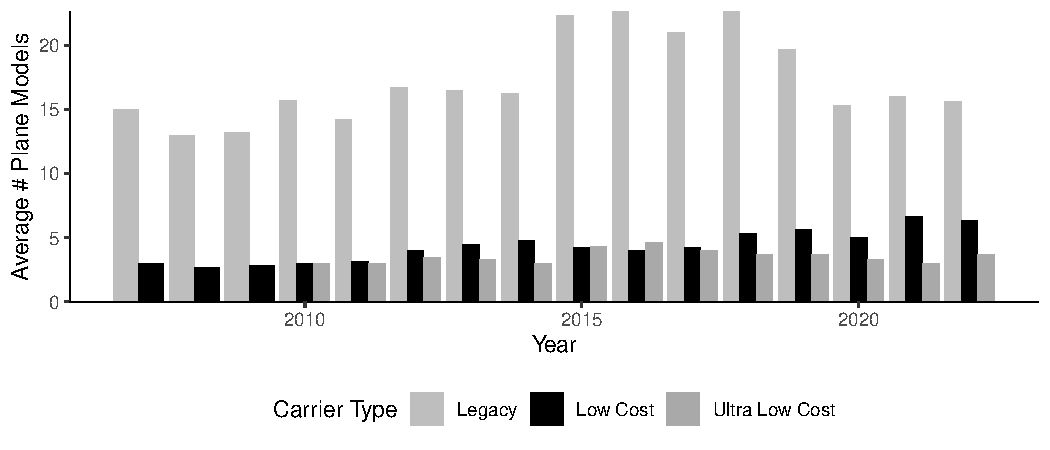
\includegraphics[width = \linewidth]{average_plane_types_in_use.pdf}
		\footnotesize{Source: B-43 Inventory Data. Legacy Carriers are Delta Air Lines, American Airlines, US Airways, and United Air Lines. Low Cost Carriers are Virgin America, JetBlue Airways, Southwest Airlines, and Alaska Airlines. Ultra Low Cost Carriers are Spirit Air Lines, Allegiant Air, and Frontier Airlines. Ultra Low Cost Carriers are included as LCC until they adopt the ULCC business model in  2010,  2012, and  2013 respectively.}
	\end{figure}
	
	\begin{figure}
		\caption{Ultra-Low Cost Carrier Share of Trips}
		\label{fig:ULCC_Trips}
		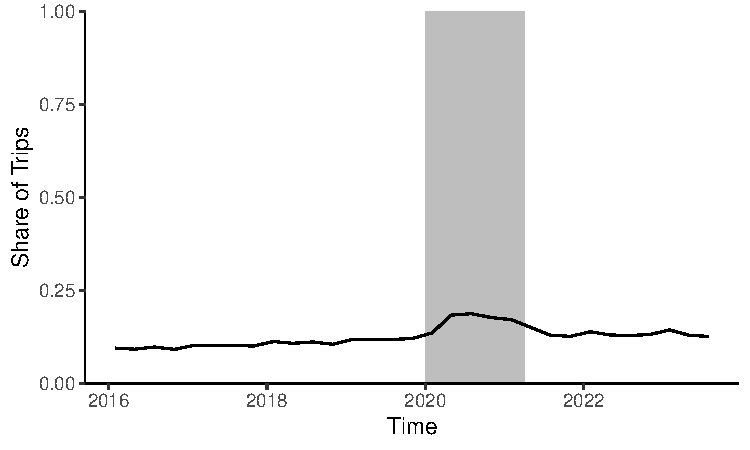
\includegraphics[width = \linewidth]{ULCC_Share}
		\footnotesize{Derived from DB1B data. Ultra-Low Cost Carriers are Spirit, Frontier, and Allegiant. Shaded region depicts the duration of the coronavirus pandemic before widespread vaccine availability within the United States. Unidirectional trips are plotted, as such, a round-way trip is counted twice.}
	\end{figure}
	
	\begin{figure}[h]
		\caption{Big Four Ridership Over Time}
		\label{fig:BigFour_Ridership}
		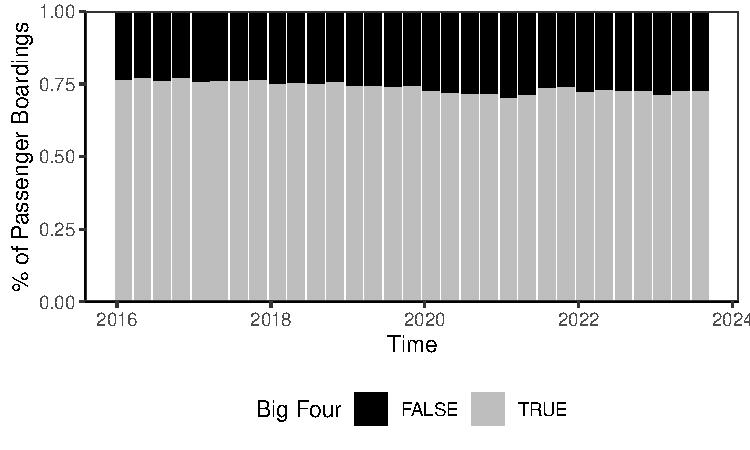
\includegraphics{BigFour_Ridership_Graph.pdf}
		\footnotesize{Derived from DB1B data. The "Big Four" carriers are the legacy carriers Delta, United, and American as well as the largest low-cost carrier, Southwest Airlines.}
	\end{figure}

\begin{figure}
	\caption{Jet Fuel Price, By Firm}
	\label{fig:JetFuel}
	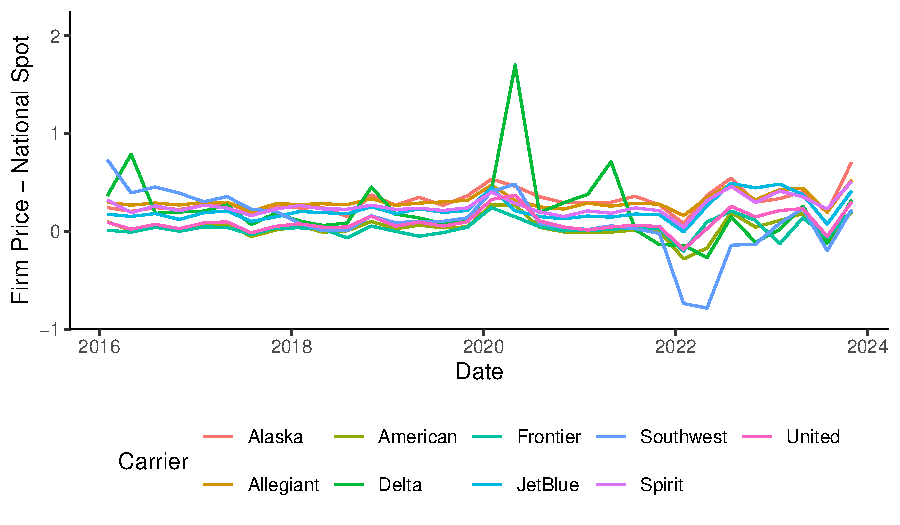
\includegraphics[width = \linewidth]{Fuel_Price_Compare}
	\footnotesize{Source: Schedule P-12 Financial Filings, Energy Information Administration Jet Fuel Spot Price Time Series. Each line is the difference between the reported quarterly expenditure on fuel for each firm and the national average spot price of oil within the quarter.}
\end{figure}

\begin{figure}
	\caption{Number of Low Cost, Ultra-Low Cost Carriers in Each Market}
	\label{fig:LCC_Count}
	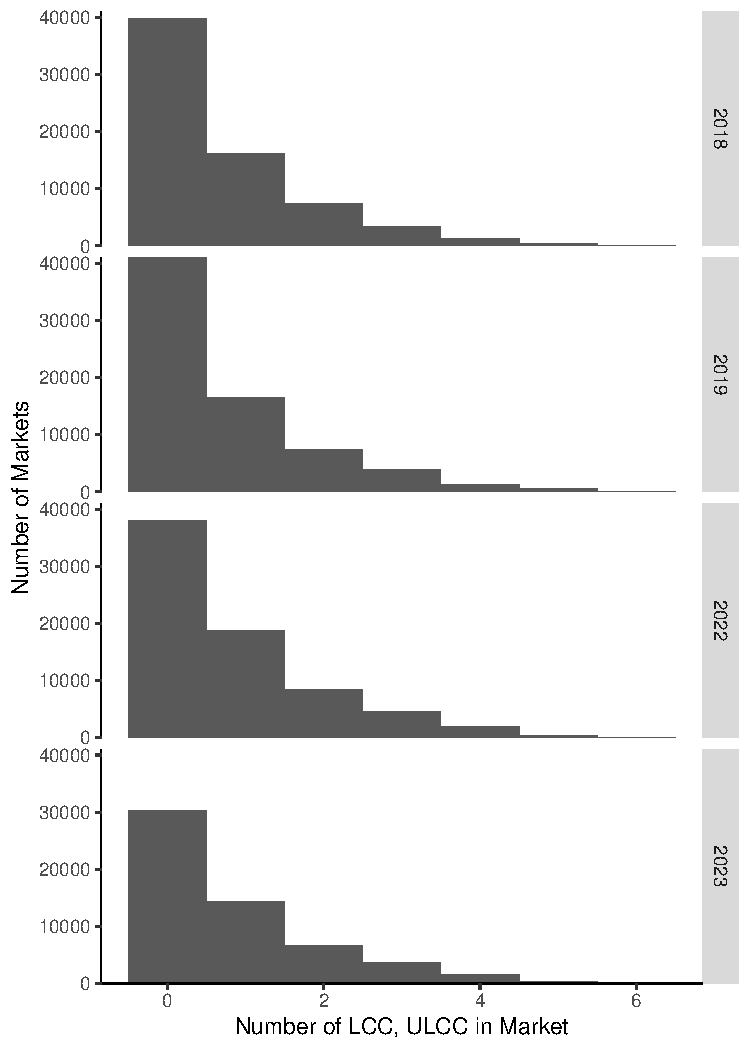
\includegraphics[width = \linewidth]{LCC_Density}
	\footnotesize{Source: DB1B Data. Markets are defined as a set of Year, Quarter, Origin Airport, and Destination Airport. Within this graph, only the major low-cost and ultra-low cost carriers are graphed (Southwest, JetBlue, Alaska, Hawaiian, Spirit, Allegiant, Frontier).}
\end{figure}

\begin{figure}
	\caption{Quarterly Passengers, All Carriers}
	\label{fig:QuarterlyPass}
	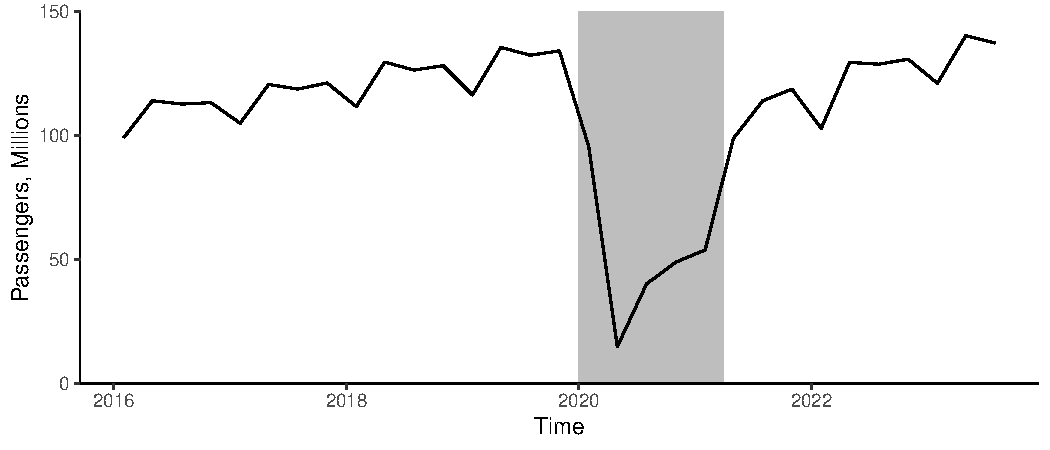
\includegraphics[width = \linewidth]{Quarterly_DB1B_Itineraries}
	\footnotesize{Source: DB1B Data. Shaded region depicts the duration of the coronavirus pandemic before widespread vaccine availability within the United States, namely, from the first quarter of 2020 through the first quarter of 2021.}
\end{figure}

\FloatBarrier

	\subsection{Descriptive Figures and Tables: Northeast Alliance}

			\begin{table}[h]
		\caption{Northeast Alliance Timeline}
		\label{tab:NEA_Timeline}
		\begin{center}
			\begin{tabular}{ccc}
				\hline
				Year & Date & Event \\
				\hline
				2020 & Quarter 1-2 & JetBlue and American Negotiate Alliance \\ 
				& July 16 & Northeast Alliance Announced \\
				& July 22 & Alliance Agreement submitted to DOT \\
				\hline 
				2021 & January 10 & DOT Terminates Antitrust Review \\
				& February 24 & Codesharing Agreement Begins on {X} Routes \\
				& May 26 & Reciprocal Loyalty Earnings Begins \\
				& Early September & NEA Shuttle at JFK Opens \\
				& September 21 & DOJ Files Lawsuit Against NEA \\  
				\hline
				2022 & September 27 - November 18 & NEA-Trial \\
				\hline 
				2023 & May 19 & NEA Ruled Anticompetitive \\
				& July 5 & JetBlue Drops Appeal Plans \\
				& July 21 & NEA Codesharing Ends \\
				& October 31 & JFK Shuttle Ceases Operation\\
				& October 31 & 12 Slot Leases to JetBlue Terminate \\
				\hline 
				2024 &  March 31  & 27 Slot Leases to JetBlue Terminate \\ 
				& March 31 & 1 Slot Lease to American Terminates \\
				& October 26 & Remaining NEA Slot Leases Terminate				 \end{tabular}
		\end{center}
	\end{table}
	
	
	\begin{table}[h]
		\caption{American, JetBlue Overlap at NEA Airports}
		\label{tab:NEA_Airport_Prescence}
		
\begin{tabular}[t]{rrrrrrrrr}
\toprule
\multicolumn{1}{c}{ } & \multicolumn{2}{c}{JFK} & \multicolumn{2}{c}{BOS} & \multicolumn{2}{c}{LGA} & \multicolumn{2}{c}{EWR} \\
\cmidrule(l{3pt}r{3pt}){2-3} \cmidrule(l{3pt}r{3pt}){4-5} \cmidrule(l{3pt}r{3pt}){6-7} \cmidrule(l{3pt}r{3pt}){8-9}
Year & Ticket & Operating & Ticket & Operating & Ticket & Operating & Ticket & Operating\\
\midrule
\addlinespace[0.3em]
\multicolumn{9}{l}{\textbf{Q1}}\\
\hspace{1em}2023 & 75.4 & 23.7 & 69.1 & 21.4 & 67.3 & 4.2 & 46.7 & 7.7\\
\hspace{1em}2022 & 77.0 & 29.7 & 75.0 & 29.1 & 73.9 & 8.9 & 47.6 & 8.3\\
\hspace{1em}2021 & 18.6 & 24.4 & 26.8 & 21.7 & 50.0 & 33.3 & 9.5 & 13.6\\
\hspace{1em}2019 & 22.4 & 23.3 & 22.9 & 20.0 & 8.1 & 6.7 & 0.0 & 0.0\\
\addlinespace[0.3em]
\multicolumn{9}{l}{\textbf{Q2}}\\
\hspace{1em}2023 & 70.0 & 15.9 & 63.1 & 22.2 & 68.3 & 5.4 & 46.7 & 7.7\\
\hspace{1em}2022 & 68.3 & 26.5 & 70.3 & 21.9 & 75.0 & 6.4 & 45.5 & 17.4\\
\hspace{1em}2021 & 57.7 & 21.1 & 57.4 & 28.6 & 27.3 & 7.4 & 28.6 & 13.6\\
\hspace{1em}2019 & 21.1 & 21.0 & 21.2 & 25.0 & 8.9 & 5.6 & 0.0 & 0.0\\
\addlinespace[0.3em]
\multicolumn{9}{l}{\textbf{Q3}}\\
\hspace{1em}2023 & 69.0 & 16.9 & 63.9 & 19.0 & 61.0 & 4.1 & 40.0 & 7.7\\
\hspace{1em}2022 & 73.8 & 21.9 & 73.8 & 24.2 & 75.9 & 6.4 & 57.1 & 7.1\\
\hspace{1em}2021 & 63.6 & 25.9 & 58.9 & 23.1 & 30.4 & 3.2 & 37.5 & 14.8\\
\hspace{1em}2019 & 19.6 & 20.3 & 21.6 & 21.6 & 8.9 & 5.6 & 0.0 & 0.0\\
\addlinespace[0.3em]
\multicolumn{9}{l}{\textbf{Q4}}\\
\hspace{1em}2022 & 72.1 & 25.4 & 66.1 & 21.1 & 69.8 & 2.0 & 46.7 & 7.7\\
\hspace{1em}2021 & 71.9 & 25.8 & 73.2 & 23.2 & 75.0 & 4.3 & 43.5 & 7.7\\
\hspace{1em}2019 & 15.3 & 17.5 & 22.0 & 19.2 & 6.8 & 5.4 & 0.0 & 0.0\\
\bottomrule
\end{tabular}

		\footnotesize{Each cell is the percent of markets originating from the specified airport with both carriers present in the market as ticket issuing carriers or the carrier who operated flights within the market.}
	\end{table}
	
	\begin{landscape}
		\begin{table}
			\caption{Exposure to Northeast Alliance}
			\label{tab:NEA_Exposure}
			\include{06.Tables/NEA_Percentage_Tied_Up}
			\begin{minipage}{1.75\textwidth} % choose width suitably
				{\footnotesize A "NEA Route" is a direct flight with either origin or destination that is BOS, JFK, LGA, EWR. "\% NEA Passengers" refers to the share of an airline's passengers that had itinerary with origin, destination, or intermediate stop at one of BOS, JFK, LGA, EWR. "\% NEA Revenues"  is the percentage of an airline's revenue within the domestic United States generated by the aforementioned passengers, calculated by multiplying the number of passengers of an itinerary by its average fare. It does not account for inter firm transfers in the case of JetBlue and American.}
			\end{minipage}
		\end{table}
	\end{landscape}
	
		\begin{figure}
		\caption{American-JetBlue Joint Itinerary}
		\label{fig:NEA_Joint_Op}
		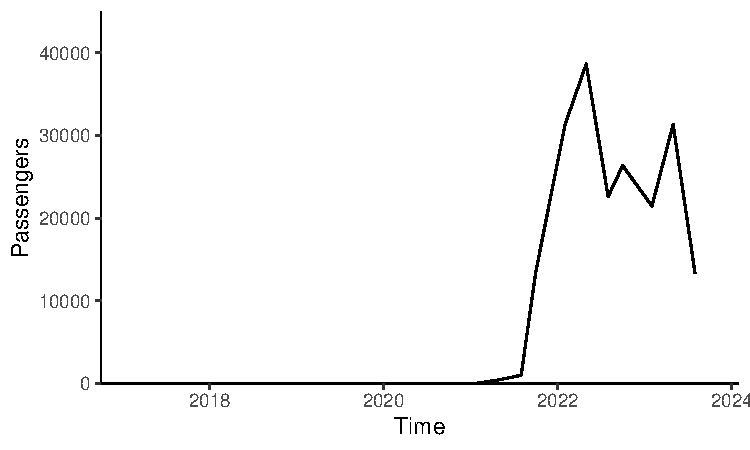
\includegraphics[width = \linewidth]{NEA_OPCarrier_Switch_Graph}
		\begin{minipage}{\textwidth} % choose width suitably
			{\footnotesize This figure plots ten times the number of passengers recorded in the DB1B who flew on an itinerary with two legs that includes both JetBlue and American as the operating carriers.}
		\end{minipage}
	\end{figure}
	
	
	\begin{figure}
		\caption{American Ticket, JetBlue Operated}
		\label{fig:NEA_Mix_AAB6}
		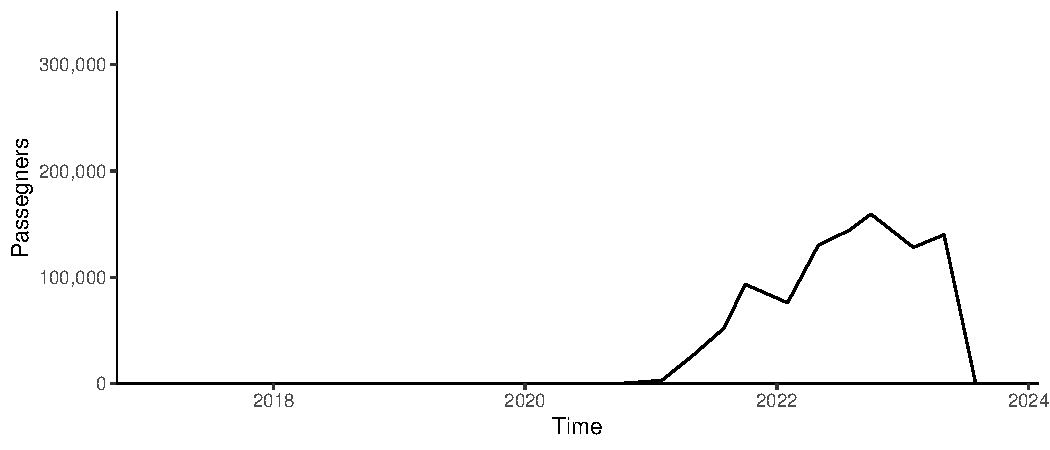
\includegraphics[width = \linewidth]{NEA_AATk_B6Op.pdf}
		\begin{minipage}{\textwidth} % choose width suitably
			{\footnotesize This figure plots ten times the number of passengers recorded in the DB1B who flew on an itinerary with American indicated as the ticketing carrier and JetBlue indicated as the operating carrier for at least one leg of the journey. Only itineraries with one layover or fewer are included. }
		\end{minipage}
	\end{figure}
	
	\begin{figure}
		\caption{JetBlue Ticket, American Operated}
		\label{fig:NEA_Mix_B6AA}
		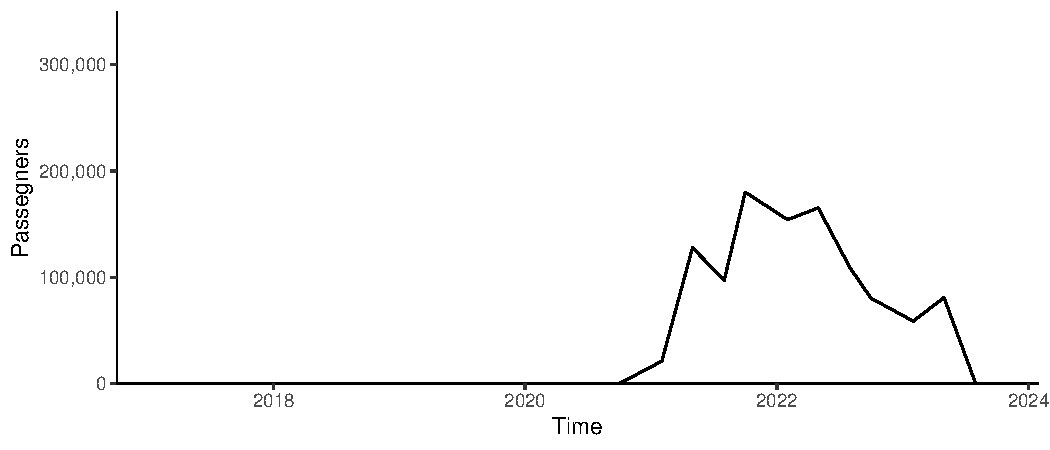
\includegraphics[width = \linewidth]{NEA_B6TK_AAOp.pdf}
		\begin{minipage}{\textwidth} % choose width suitably
			{\footnotesize This figure plots ten times the number of passengers recorded in the DB1B who flew on an itinerary with JetBlue indicated as the ticketing carrier and American indicated as the operating carrier for at least one leg of the journey. Only itineraries with one layover or fewer are included. }
		\end{minipage}
	\end{figure}
	


\FloatBarrier
	
	\subsection{Descriptive Figures and Tables: JetBlue, Spirit}

	
	\begin{table}[h]
		\caption{JetBlue-Spirit Merger Timeline}
		\label{tab:JetBlue_Spirit_Timeline}
		\begin{center}
			\begin{tabular}{ccc}
				\hline
				Year & Date & Event \\
				\hline
				2022 & February 7 & Frontier-Spirit Merger Announced \\
				& April 5 &  First JetBlue Offer for Spirit Released\\
				& May 6 & Spirit Rejects JetBlue Offer \\
				& July 27 &  Frontier-Spirit Merger Attempt Collapses\\
				& July 28 &  Spirit Board Approves JetBlue Merger\\
				& October 19 & Spirit Shareholders Approve Merger \\
				\hline
				2023 & March 7 &  Department of Justice Files Suit\\
				& October 31 - December 5 &  JetBlue-Spirit Merger Trial \\
				\hline
				2024 & January 16 & JetBlue-Spirit Merger Blocked \\
				& March 4 & JetBlue, Spirit Drop Appeal Plans \\
			\end{tabular}
		\end{center}
	\end{table}

	\begin{figure}
	\caption{Spirit Fleet Size Over Time}
	\label{fig:Spirit_fleet}
	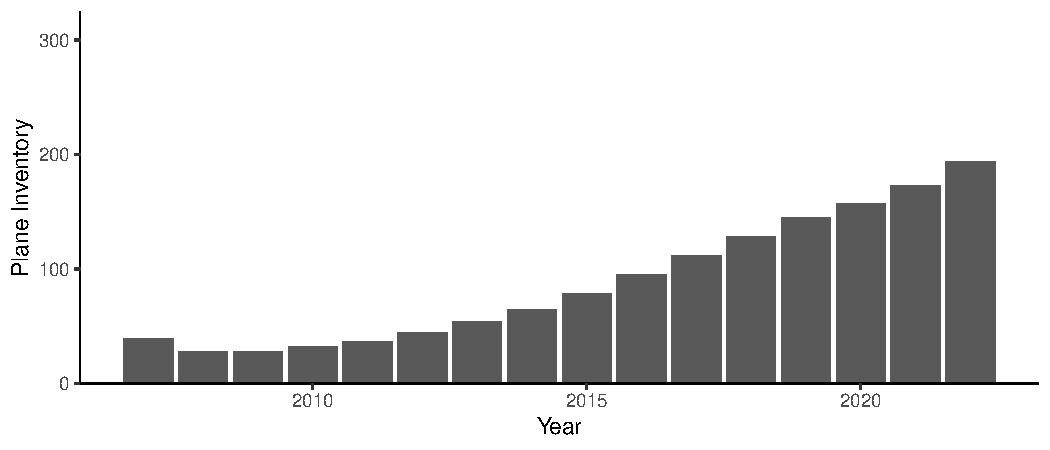
\includegraphics[width = \linewidth]{Spirit_Planes.pdf}
	\footnotesize{Source: B-43 Inventory Data. Each bar is the number of airplanes in Spirit's inventory within a given year. }
\end{figure}

\begin{figure}
	\caption{JetBlue Fleet Size Over Time}
	\label{fig:JetBlue_Fleet}
	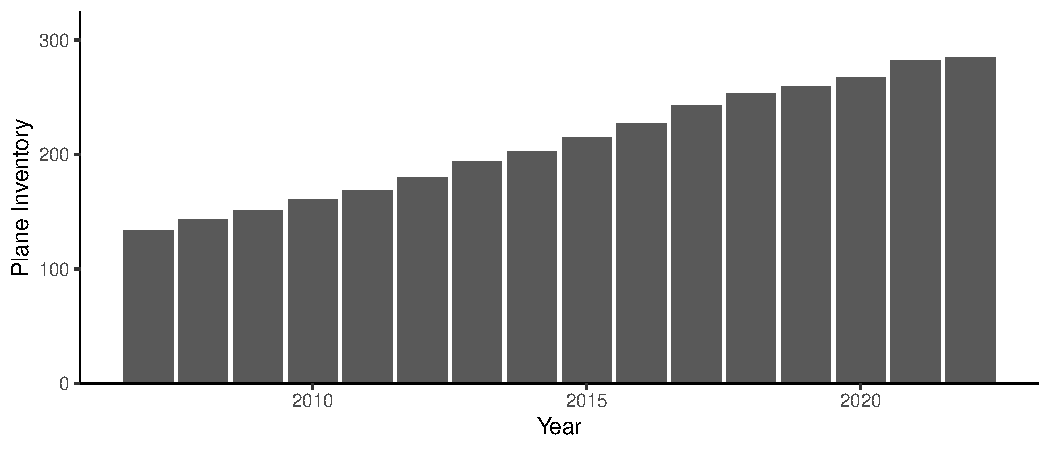
\includegraphics[width = \linewidth]{JetBlue_Planes.pdf}
	\footnotesize{Source: B-43 Inventory Data. Each bar is the number of airplanes in Spirit's inventory within a given year.}
\end{figure}

\begin{figure}
	\caption{JetBlue, Spirit Airports - 2012}
	\label{fig:JBSpirit_Airports_2012}
	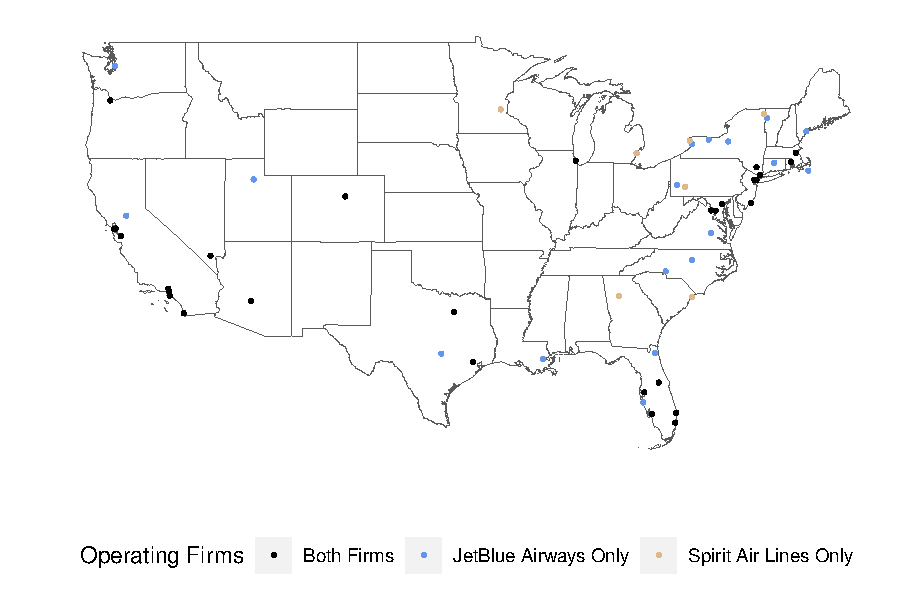
\includegraphics[width = \linewidth]{Map_Mainland_Both_2012.pdf}
	\footnotesize{Derived from DB1B Data. Beyond the United States mainland, both carriers operated in Puerto Rico.}
\end{figure}

\begin{figure}
	\caption{JetBlue, Spirit Airports - 2022}
	\label{fig:JBSpirit_Airports_2022}
	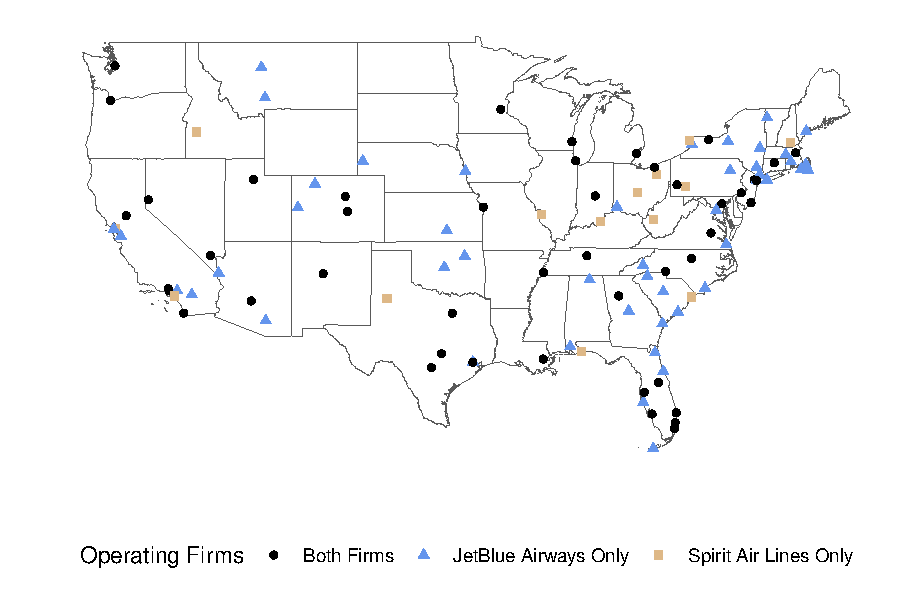
\includegraphics[width = \linewidth]{Map_Mainland_Both_2022.pdf}
	\footnotesize{Derived from DB1B Data. Beyond the United States mainland, both carriers operated in Puerto Rico.}
\end{figure}

\begin{table}
	\begin{center}
		\caption{JetBlue, Spirit Fleet Composition - 2022}
		\label{tab:JetBlueSpirit_Fleet}
		
\begin{tabular}[t]{llrrr}
\toprule
Manufacturer & Model & Seats & Count & Total Seats\\
\midrule
\addlinespace[0.3em]
\multicolumn{5}{l}{\textbf{JetBlue}}\\
\hspace{1em}Airbus & A220 & 140 & 14 & 1960\\
\hspace{1em}Airbus & A320 & 150 & 11 & 1650\\
\hspace{1em}Airbus & A320 & 162 & 119 & 19278\\
\hspace{1em}Airbus & A321 & 159 & 35 & 5565\\
\hspace{1em}Airbus & A321 & 200 & 28 & 5600\\
\hspace{1em}Airbus & A321neo & 138 & 5 & 690\\
\hspace{1em}Airbus & A321neo & 160 & 2 & 320\\
\hspace{1em}Airbus & A321neo & 200 & 16 & 3200\\
\hspace{1em}Embraer & E190 & 100 & 55 & 5500\\
\addlinespace[0.3em]
\multicolumn{5}{l}{\textbf{Spirit}}\\
\hspace{1em}Airbus & A319 & 145 & 31 & 4495\\
\hspace{1em}Airbus & A320 & 182 & 133 & 24206\\
\hspace{1em}Airbus & A321 & 228 & 30 & 6840\\
\bottomrule
\end{tabular}

	\end{center}
	\footnotesize{Source: B-43 Inventory Data. }
\end{table}

	\begin{table}
		\caption{JetBlue and Spirit: Overlap Cities - 2022}
		\label{tab:KeyCities}
		
\begin{tabular}{lrrr}
\toprule
City & Firm Passengers & Total Passengers & Share\\
\midrule
Ponce, PR & 106320 & 106320 & 1.000\\
Aguadilla, PR & 251180 & 321170 & 0.782\\
San Juan, PR & 1848180 & 4149260 & 0.445\\
Boston, MA & 4262240 & 12136460 & 0.351\\
West Palm Beach/Palm Beach, FL & 919690 & 2960650 & 0.311\\
\addlinespace
Miami, FL & 5885260 & 19049140 & 0.309\\
Charlotte Amalie, VI & 155220 & 584450 & 0.266\\
New York, NY & 8243150 & 32401400 & 0.254\\
Hartford, CT & 596840 & 2358950 & 0.253\\
Orlando, FL & 4890200 & 19981730 & 0.245\\
\addlinespace
Fort Myers, FL & 964970 & 4577540 & 0.211\\
Detroit, MI & 1330090 & 7481070 & 0.178\\
Cleveland, OH & 567000 & 3537960 & 0.160\\
Richmond, VA & 235760 & 1474130 & 0.160\\
New Orleans, LA & 774190 & 4909390 & 0.158\\
\addlinespace
Las Vegas, NV & 2783710 & 18384770 & 0.151\\
Tampa, FL & 1371860 & 9955070 & 0.138\\
Pittsburgh, PA & 391900 & 3023570 & 0.130\\
Los Angeles, CA & 2839960 & 22400620 & 0.127\\
Philadelphia, PA & 844170 & 7694760 & 0.110\\
\bottomrule
\end{tabular}

		\footnotesize{Derived from DB1B Data. Cities are ordered by the combined share of passengers who used JetBlue or Spirit flights as a share of the total passengers departing from the city within 2022. Cities in which only one firm operates are excluded.}
	\end{table}

	
	\FloatBarrier
	
	\subsection{Estimation Results: Northeast Alliance}

	\begin{table}
	\caption{Probability of American, JetBlue Operating Switch}
	\label{tab:NEA_Switch_Prob}
	
\begin{tabular}{l c}
\hline
 & Model 1 \\
\hline
(Intercept)          & $0.00000 \; (0.00000)$ \\
NEA\_Market          & $0.00000 \; (0.00000)$ \\
NEA\_Market:Period-8 & $0.00000 \; (0.00000)$ \\
NEA\_Market:Period-7 & $0.00000 \; (0.00000)$ \\
NEA\_Market:Period-6 & $0.00000 \; (0.00000)$ \\
NEA\_Market:Period-5 & $0.00000 \; (0.00000)$ \\
NEA\_Market:Period-4 & $0.00000 \; (0.00000)$ \\
NEA\_Market:Period-3 & $0.00000 \; (0.00000)$ \\
NEA\_Market:Period-2 & $0.00000 \; (0.00000)$ \\
NEA\_Market:Period0  & $0.00000 \; (0.00000)$ \\
NEA\_Market:Period1  & $0.00000 \; (0.00000)$ \\
NEA\_Market:Period2  & $0.00000 \; (0.00000)$ \\
NEA\_Market:Period3  & $0.00000 \; (0.00000)$ \\
NEA\_Market:Period4  & $0.00000 \; (0.00000)$ \\
NEA\_Market:Period5  & $0.00000 \; (0.00000)$ \\
NEA\_Market:Period6  & $0.00000 \; (0.00000)$ \\
NEA\_Market:Period7  & $0.00000 \; (0.00000)$ \\
NEA\_Market:Period8  & $0.00000 \; (0.00000)$ \\
\hline
R$^2$                & $$                     \\
Adj. R$^2$           & $$                     \\
Num. obs.            & $84533$                \\
\hline
\multicolumn{2}{l}{\scriptsize{$^{***}p<0.01$; $^{**}p<0.05$; $^{*}p<0.1$}}
\end{tabular}

	\footnotesize{Dependent variable is the probability that within a market, at least one passenger took planes operated by both American and JetBlue as part of their itinerary. Base period is 2021 Quarter 2. All data from 2020 and the first quarter of 2021 is excluded , as such,  Period -1 is the fourth quarter of 2019.Standard errors are clustered at the level of origin, destination airport pairs.}
\end{table}
	
	\begin{figure}
		\caption{Probability of American, JetBlue Codeshares Observed}
		\label{tab:NEA_Switch_Graph}
		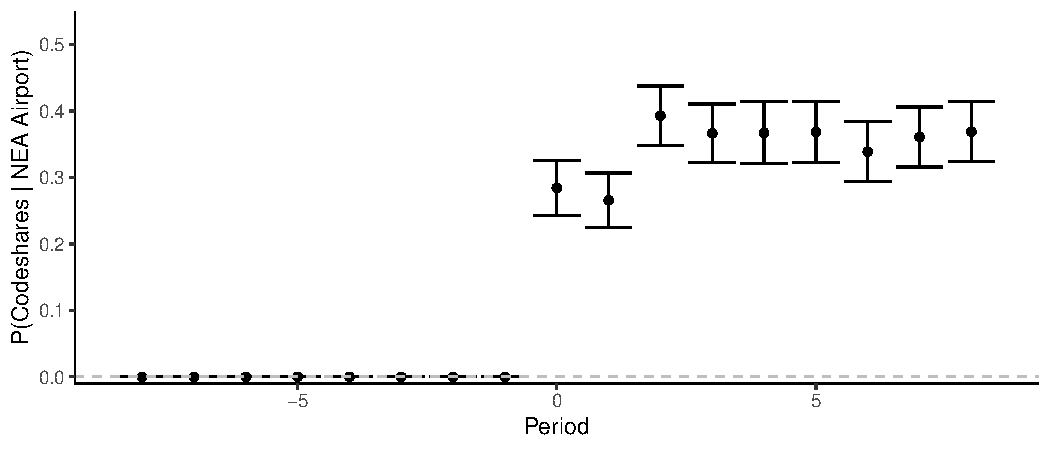
\includegraphics[width = \linewidth]{NEA_Probability_Switches_Graph}
		\footnotesize{Figure plots the estimated event study coefficients from Table \ref{tab:NEA_Switch_Prob}. Dependent variable is the probability that within a market, at least one passenger took planes operated by both American and JetBlue as part of their itinerary. Base period is 2021 Quarter 2. All data from 2020 and the first quarter of 2021 is excluded , as such,  Period -1 is the fourth quarter of 2019.}
	\end{figure}
	
	\begin{table}
		\caption{American, JetBlue Fare Difference}
		\label{tab:NEA_Fare_Neutral}
		
\begin{tabular}{l c c c c c}
\hline
 & Model 1 & Model 2 & Model 3 & Model 4 & Model 5 \\
\hline
NEA\_Market:Period-8 & $-0.26906$        & $0.30596$         &                  & $-0.29184$        &                  \\
                     & $(5.75228)$       & $(5.77309)$       &                  & $(5.75995)$       &                  \\
NEA\_Market:Period-7 & $5.09132$         & $5.67806$         &                  & $5.13022$         &                  \\
                     & $(5.17678)$       & $(5.22338)$       &                  & $(5.19612)$       &                  \\
NEA\_Market:Period-6 & $10.03942^{*}$    & $10.63729^{**}$   &                  & $10.14576^{*}$    &                  \\
                     & $(5.35652)$       & $(5.38161)$       &                  & $(5.37598)$       &                  \\
NEA\_Market:Period-5 & $11.76106^{**}$   & $12.00179^{**}$   &                  & $11.84893^{**}$   &                  \\
                     & $(4.92281)$       & $(4.93152)$       &                  & $(4.93757)$       &                  \\
NEA\_Market:Period-4 & $2.18901$         & $2.13655$         & $1.98855$        & $2.14272$         & $1.95626$        \\
                     & $(5.58228)$       & $(5.58620)$       & $(5.59391)$      & $(5.57950)$       & $(5.59321)$      \\
NEA\_Market:Period-3 & $19.12171^{***}$  & $19.10709^{***}$  & $19.07312^{***}$ & $19.35021^{***}$  & $19.47877^{***}$ \\
                     & $(5.73553)$       & $(5.71661)$       & $(5.72866)$      & $(5.75325)$       & $(5.76216)$      \\
NEA\_Market:Period-2 & $6.44965$         & $6.67093$         & $6.51433$        & $6.53793$         & $6.69157$        \\
                     & $(5.83867)$       & $(5.83683)$       & $(5.84524)$      & $(5.85405)$       & $(5.85874)$      \\
NEA\_Market:Period0  & $-7.25121$        & $-6.75069$        & $-7.08500$       & $-7.16336$        & $-7.06777$       \\
                     & $(6.41124)$       & $(6.41684)$       & $(6.42156)$      & $(6.41050)$       & $(6.41885)$      \\
NEA\_Market:Period1  & $7.49030$         & $8.20226$         & $7.10715$        & $7.62169$         & $6.14813$        \\
                     & $(5.86068)$       & $(5.85658)$       & $(5.90042)$      & $(5.85369)$       & $(5.88378)$      \\
NEA\_Market:Period2  & $-4.28124$        & $-2.06886$        & $-2.11545$       & $-4.84285$        & $-3.70597$       \\
                     & $(5.97452)$       & $(5.95494)$       & $(5.93054)$      & $(5.95360)$       & $(5.92021)$      \\
NEA\_Market:Period3  & $6.88578$         & $8.00691$         & $6.39743$        & $6.51208$         & $3.90301$        \\
                     & $(5.91318)$       & $(5.88990)$       & $(5.93723)$      & $(5.90607)$       & $(5.92192)$      \\
NEA\_Market:Period4  & $-27.21576^{***}$ & $-25.74536^{***}$ &                  & $-27.46203^{***}$ &                  \\
                     & $(5.80239)$       & $(5.80982)$       &                  & $(5.80723)$       &                  \\
NEA\_Market:Period5  & $-26.01830^{***}$ & $-24.31807^{***}$ &                  & $-26.10865^{***}$ &                  \\
                     & $(5.61729)$       & $(5.62150)$       &                  & $(5.60841)$       &                  \\
NEA\_Market:Period6  & $-48.46402^{***}$ & $-47.36784^{***}$ &                  & $-48.99718^{***}$ &                  \\
                     & $(5.71876)$       & $(5.70989)$       &                  & $(5.71473)$       &                  \\
NEA\_Market:Period7  & $-47.09005^{***}$ &                   &                  & $-47.65451^{***}$ &                  \\
                     & $(5.89402)$       &                   &                  & $(5.89024)$       &                  \\
NEA\_Market:Period8  & $-45.42148^{***}$ &                   &                  & $-46.27267^{***}$ &                  \\
                     & $(5.59951)$       &                   &                  & $(5.57531)$       &                  \\
\hline
Standard Controls    & Yes               & Yes               & Yes              & Yes               & Yes              \\
Income Data          &                   & MSA               & MSA              & State             & State            \\
Sample               & Full              & Full              & Two Years        & Full              & Two Years        \\
R$^2$                & $0.09762$         & $0.07689$         & $0.03263$        & $0.10155$         & $0.04425$        \\
Adj. R$^2$           & $0.09545$         & $0.07449$         & $0.02960$        & $0.09933$         & $0.04127$        \\
Num. obs.            & $15838$           & $13534$           & $6712$           & $15838$           & $6748$           \\
\hline
\multicolumn{6}{l}{\scriptsize{$^{***}p<0.01$; $^{**}p<0.05$; $^{*}p<0.1$}}
\end{tabular}

		\footnotesize{Dependent variable is the difference of the average fare within a market of American Airlines less the average fare of JetBlue. Base period is 2021 Quarter 2. All data from 2020 and the first quarter of 2021 is excluded , as such,  Period -1 is the fourth quarter of 2019. Standard errors are clustered at the level of origin, destination airport pairs.}
	\end{table}
	
	\begin{figure}
		\caption{American, JetBlue Fare Difference}
		\label{fig:NEA_Fare_Neutral}
		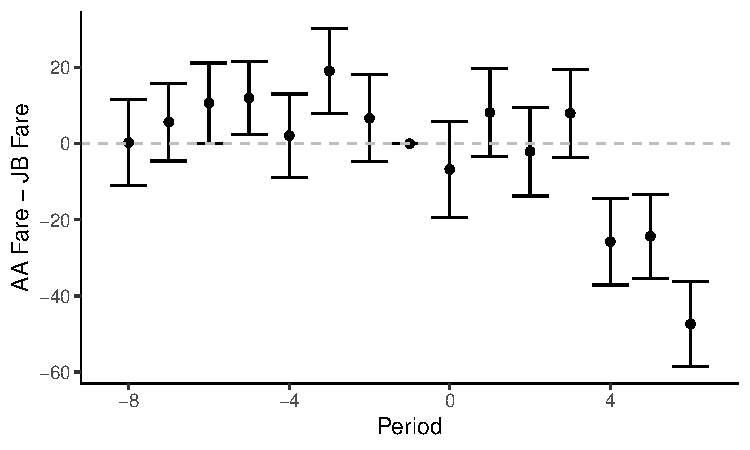
\includegraphics[width = \linewidth]{NEA_Price_Neutrality_Graph}
		\footnotesize{Figure plots the estimated event study coefficients from Table \ref{tab:NEA_Fare_Neutral} Base period is 2021 Quarter 2. All data from 2020 and the first quarter of 2021 is excluded , as such,  Period -1 is the fourth quarter of 2019.}
	\end{figure}
	
	\begin{table}
		\caption{American, JetBlue Yield Difference}
		\label{tab:NEA_Yield_Neutral}
		
\begin{tabular}{l c c c c c}
\hline
 & Model 1 & Model 2 & Model 3 & Model 4 & Model 5 \\
\hline
NEA\_Market:Period-8 & $0.00726$        & $0.00694$        &                 & $0.00725$        &                 \\
                     & $(0.00579)$      & $(0.00576)$      &                 & $(0.00578)$      &                 \\
NEA\_Market:Period-7 & $0.01378^{**}$   & $0.01326^{**}$   &                 & $0.01381^{**}$   &                 \\
                     & $(0.00595)$      & $(0.00591)$      &                 & $(0.00594)$      &                 \\
NEA\_Market:Period-6 & $0.01266^{**}$   & $0.01191^{**}$   &                 & $0.01274^{**}$   &                 \\
                     & $(0.00549)$      & $(0.00545)$      &                 & $(0.00549)$      &                 \\
NEA\_Market:Period-5 & $0.00666$        & $0.00642$        &                 & $0.00672$        &                 \\
                     & $(0.00515)$      & $(0.00513)$      &                 & $(0.00514)$      &                 \\
NEA\_Market:Period-4 & $0.00219$        & $0.00197$        & $0.00220$       & $0.00215$        & $0.00234$       \\
                     & $(0.00478)$      & $(0.00475)$      & $(0.00477)$     & $(0.00478)$      & $(0.00480)$     \\
NEA\_Market:Period-3 & $0.00695$        & $0.00684$        & $0.00698$       & $0.00712$        & $0.00728$       \\
                     & $(0.00463)$      & $(0.00462)$      & $(0.00463)$     & $(0.00462)$      & $(0.00463)$     \\
NEA\_Market:Period-2 & $0.00886^{*}$    & $0.00859^{*}$    & $0.00858^{*}$   & $0.00892^{*}$    & $0.00892^{*}$   \\
                     & $(0.00508)$      & $(0.00505)$      & $(0.00506)$     & $(0.00507)$      & $(0.00507)$     \\
NEA\_Market:Period0  & $0.00933^{*}$    & $0.00886^{*}$    & $0.00954^{*}$   & $0.00939^{*}$    & $0.01012^{*}$   \\
                     & $(0.00532)$      & $(0.00527)$      & $(0.00526)$     & $(0.00532)$      & $(0.00529)$     \\
NEA\_Market:Period1  & $0.02109^{***}$  & $0.02124^{***}$  & $0.02080^{***}$ & $0.02119^{***}$  & $0.02065^{***}$ \\
                     & $(0.00537)$      & $(0.00531)$      & $(0.00529)$     & $(0.00535)$      & $(0.00531)$     \\
NEA\_Market:Period2  & $0.01420^{***}$  & $0.01417^{***}$  & $0.01564^{***}$ & $0.01379^{**}$   & $0.01521^{***}$ \\
                     & $(0.00539)$      & $(0.00536)$      & $(0.00535)$     & $(0.00539)$      & $(0.00536)$     \\
NEA\_Market:Period3  & $0.01652^{***}$  & $0.01754^{***}$  & $0.01642^{***}$ & $0.01624^{***}$  & $0.01494^{***}$ \\
                     & $(0.00547)$      & $(0.00541)$      & $(0.00541)$     & $(0.00545)$      & $(0.00543)$     \\
NEA\_Market:Period4  & $-0.00850$       & $-0.00878^{*}$   &                 & $-0.00868$       &                 \\
                     & $(0.00530)$      & $(0.00529)$      &                 & $(0.00529)$      &                 \\
NEA\_Market:Period5  & $-0.00560$       & $-0.00544$       &                 & $-0.00566$       &                 \\
                     & $(0.00531)$      & $(0.00531)$      &                 & $(0.00530)$      &                 \\
NEA\_Market:Period6  & $-0.02115^{***}$ & $-0.02175^{***}$ &                 & $-0.02154^{***}$ &                 \\
                     & $(0.00585)$      & $(0.00586)$      &                 & $(0.00586)$      &                 \\
NEA\_Market:Period7  & $-0.02522^{***}$ &                  &                 & $-0.02563^{***}$ &                 \\
                     & $(0.00588)$      &                  &                 & $(0.00590)$      &                 \\
NEA\_Market:Period8  & $-0.01742^{***}$ &                  &                 & $-0.01804^{***}$ &                 \\
                     & $(0.00589)$      &                  &                 & $(0.00592)$      &                 \\
\hline
Standard Controls    & Yes              & Yes              & Yes             & Yes              & Yes             \\
Income Data          &                  & MSA              & MSA             & State            & State           \\
Sample               & Full             & Full             & Two Years       & Full             & Two Years       \\
R$^2$                & $0.14162$        & $0.13168$        & $0.12855$       & $0.14334$        & $0.12850$       \\
Adj. R$^2$           & $0.13956$        & $0.12943$        & $0.12582$       & $0.14123$        & $0.12578$       \\
Num. obs.            & $15838$          & $13534$          & $6712$          & $15838$          & $6748$          \\
\hline
\multicolumn{6}{l}{\scriptsize{$^{***}p<0.01$; $^{**}p<0.05$; $^{*}p<0.1$}}
\end{tabular}

		\footnotesize{Dependent variable is the difference of the average yield within a market of American Airlines less the average yield of JetBlue. Base period is 2021 Quarter 2. All data from 2020 and the first quarter of 2021 is excluded , as such,  Period -1 is the fourth quarter of 2019. Standard errors are clustered at the level of origin, destination airport pairs.}
	\end{table}
	
	\begin{figure}
		\caption{American, JetBlue Yield Difference}
		\label{fig:NEA_Yield_Neutral}
		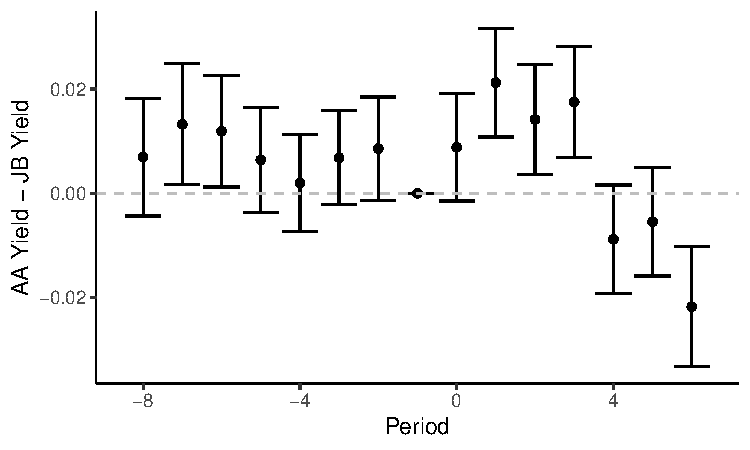
\includegraphics[width = \linewidth]{NEA_Price_Neutrality_Graph_Y}
		\footnotesize{Figure plots the estimated event study coefficients from Table \ref{tab:NEA_Yield_Neutral} Base period is 2021 Quarter 2. All data from 2020 and the first quarter of 2021 is excluded , as such,  Period -1 is the fourth quarter of 2019.}
	\end{figure}
	
	\begin{table}
		\caption{NEA Market Fare Effects}
		\label{tab:NEA_Market_Fare}
		
\begin{tabular}{l c c c c c}
\hline
 & Model 1 & Model 2 & Model 3 & Model 4 & Model 5 \\
\hline
Period-8:NEA\_Market & $-0.06122^{***}$ & $-0.06316^{***}$ &                  & $-0.06101^{***}$ &                  \\
                     & $(0.00646)$      & $(0.00671)$      &                  & $(0.00646)$      &                  \\
Period-7:NEA\_Market & $-0.01927^{***}$ & $-0.02117^{***}$ &                  & $-0.01842^{***}$ &                  \\
                     & $(0.00534)$      & $(0.00559)$      &                  & $(0.00534)$      &                  \\
Period-6:NEA\_Market & $-0.01314^{***}$ & $-0.01196^{**}$  &                  & $-0.01242^{**}$  &                  \\
                     & $(0.00490)$      & $(0.00512)$      &                  & $(0.00491)$      &                  \\
Period-5:NEA\_Market & $-0.00142$       & $-0.00124$       &                  & $-0.00136$       &                  \\
                     & $(0.00403)$      & $(0.00423)$      &                  & $(0.00404)$      &                  \\
Period-4:NEA\_Market & $-0.06271^{***}$ & $-0.06611^{***}$ & $-0.06628^{***}$ & $-0.06277^{***}$ & $-0.06320^{***}$ \\
                     & $(0.00520)$      & $(0.00546)$      & $(0.00548)$      & $(0.00521)$      & $(0.00525)$      \\
Period-3:NEA\_Market & $-0.00405$       & $-0.00701^{*}$   & $-0.00668^{*}$   & $-0.00369$       & $-0.00353$       \\
                     & $(0.00373)$      & $(0.00388)$      & $(0.00392)$      & $(0.00373)$      & $(0.00379)$      \\
Period-2:NEA\_Market & $-0.01490^{***}$ & $-0.01729^{***}$ & $-0.01718^{***}$ & $-0.01500^{***}$ & $-0.01475^{***}$ \\
                     & $(0.00363)$      & $(0.00376)$      & $(0.00380)$      & $(0.00364)$      & $(0.00367)$      \\
Period0:NEA\_Market  & $0.05228^{***}$  & $0.05472^{***}$  & $0.05803^{***}$  & $0.05115^{***}$  & $0.05473^{***}$  \\
                     & $(0.00831)$      & $(0.00849)$      & $(0.00852)$      & $(0.00832)$      & $(0.00835)$      \\
Period1:NEA\_Market  & $0.06194^{***}$  & $0.06269^{***}$  & $0.07076^{***}$  & $0.05766^{***}$  & $0.06668^{***}$  \\
                     & $(0.00724)$      & $(0.00754)$      & $(0.00755)$      & $(0.00725)$      & $(0.00724)$      \\
Period2:NEA\_Market  & $-0.02105^{***}$ & $-0.02698^{***}$ & $-0.02567^{***}$ & $-0.02321^{***}$ & $-0.02187^{***}$ \\
                     & $(0.00685)$      & $(0.00715)$      & $(0.00709)$      & $(0.00690)$      & $(0.00683)$      \\
Period3:NEA\_Market  & $-0.11727^{***}$ & $-0.12518^{***}$ & $-0.11799^{***}$ & $-0.12430^{***}$ & $-0.11633^{***}$ \\
                     & $(0.00816)$      & $(0.00851)$      & $(0.00839)$      & $(0.00834)$      & $(0.00817)$      \\
Period4:NEA\_Market  & $-0.03153^{***}$ & $-0.04249^{***}$ &                  & $-0.03621^{***}$ &                  \\
                     & $(0.00745)$      & $(0.00778)$      &                  & $(0.00753)$      &                  \\
Period5:NEA\_Market  & $-0.03405^{***}$ & $-0.04228^{***}$ &                  & $-0.04054^{***}$ &                  \\
                     & $(0.00741)$      & $(0.00772)$      &                  & $(0.00748)$      &                  \\
Period6:NEA\_Market  & $-0.02544^{***}$ & $-0.03217^{***}$ &                  & $-0.02937^{***}$ &                  \\
                     & $(0.00620)$      & $(0.00646)$      &                  & $(0.00625)$      &                  \\
Period7:NEA\_Market  & $-0.07937^{***}$ &                  &                  & $-0.08426^{***}$ &                  \\
                     & $(0.00741)$      &                  &                  & $(0.00749)$      &                  \\
Period8:NEA\_Market  & $-0.01882^{***}$ &                  &                  & $-0.02268^{***}$ &                  \\
                     & $(0.00647)$      &                  &                  & $(0.00651)$      &                  \\
\hline
Standard Controls    & Yes              & Yes              & Yes              & Yes              & Yes              \\
Income Data          &                  & MSA              & MSA              & State            & State            \\
Sample               & Full             & Full             & Two Years        & Full             & Two Years        \\
R$^2$                & $0.61326$        & $0.62880$        & $0.63120$        & $0.61787$        & $0.62754$        \\
Adj. R$^2$           & $0.61321$        & $0.62874$        & $0.63113$        & $0.61782$        & $0.62748$        \\
Num. obs.            & $315451$         & $247613$         & $135042$         & $315451$         & $149299$         \\
\hline
\multicolumn{6}{l}{\scriptsize{$^{***}p<0.01$; $^{**}p<0.05$; $^{*}p<0.1$}}
\end{tabular}

		\footnotesize{Dependent variable is the average log-market fare within a market. Base period is 2021 Quarter 2. All data from 2020 and the first quarter of 2021 is excluded , as such,  Period -1 is the fourth quarter of 2019. "Standard controls" are the log of mean population between the origin and destination metropolitan statistical areas, prescence of Spirit and Southwest, per-capita origin and destination state-level coronavirus cases, and lagged HHI. Standard errors clustered at the level of origin-destination pairs are reported.  }
	\end{table}
	
	\begin{figure}
		\caption{NEA Market Fare Graph}
		\label{fig:NEA_Market_Fare}
		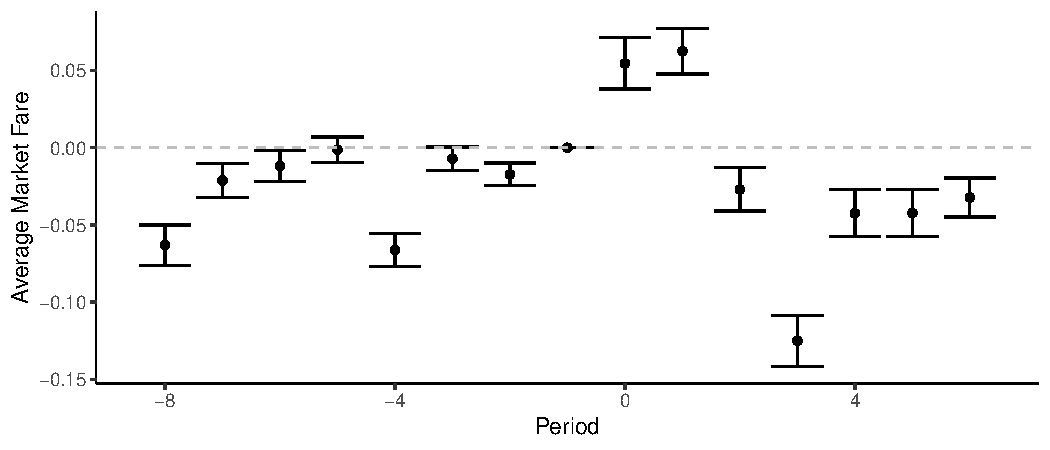
\includegraphics[width = \linewidth]{NEA_Market_Fare_Graph.pdf}
		\footnotesize{Figure plots the event study coefficients from the second column of Table \ref{tab:NEA_Market_Fare}. Base period is 2021 Quarter 2. All data from 2020 and the first quarter of 2021 is excluded, and as such, Period -1 is the fourth quarter of 2019. Standard errors clustered at the level of origin-destination pairs are reported. }
	\end{figure}
	
	\begin{figure}
		\caption{NEA Market Fare - Airport Interactions}
		\label{fig:NEA_Airport_Fare_Interaction}
		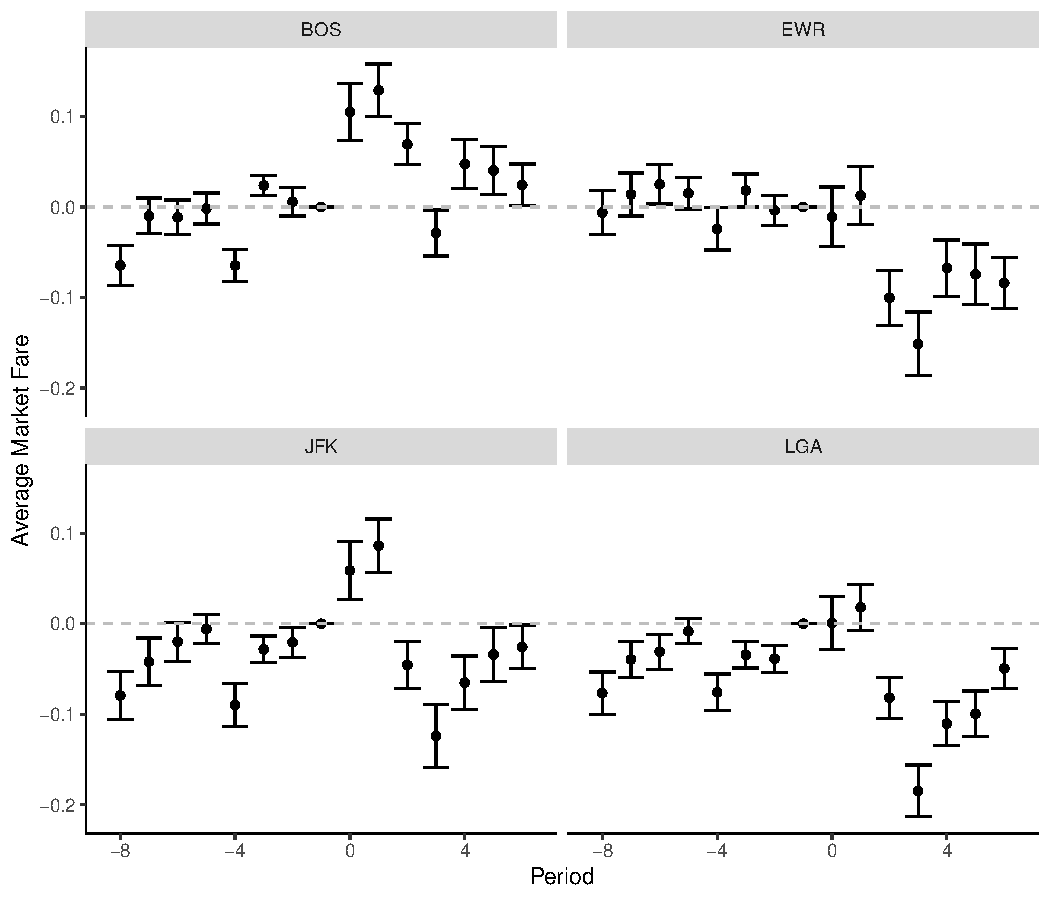
\includegraphics[width = \linewidth]{NEA_Airport_Fare_Graph}
		\footnotesize{Coefficients from a model based on the model reported in Table \ref{tab:NEA_Market_Fare} but which includes airport-time interaction terms are reported.   Base period is 2021 Quarter 2. All data from 2020 and the first quarter of 2021 is excluded, and as such, Period -1 is the fourth quarter of 2019. Standard errors clustered at the level of origin-destination pairs are reported. }
	\end{figure}
	
	\begin{table}
		\caption{NEA Market Yield Effects}
		\label{tab:NEA_Market_Yield}
		
\begin{tabular}{l c c c c c}
\hline
 & Model 1 & Model 2 & Model 3 & Model 4 & Model 5 \\
\hline
NEA Market: Period -8 & $-0.06428^{***}$ & $-0.07176^{***}$ &                  & $-0.06185^{***}$ &                  \\
                      & $(0.00922)$      & $(0.00978)$      &                  & $(0.00928)$      &                  \\
NEA Market: Period -7 & $-0.02398^{***}$ & $-0.02421^{***}$ &                  & $-0.02086^{**}$  &                  \\
                      & $(0.00832)$      & $(0.00892)$      &                  & $(0.00834)$      &                  \\
NEA Market: Period -6 & $-0.01135$       & $-0.01091$       &                  & $-0.00878$       &                  \\
                      & $(0.00743)$      & $(0.00797)$      &                  & $(0.00753)$      &                  \\
NEA Market: Period -5 & $-0.00715$       & $-0.00640$       &                  & $-0.00654$       &                  \\
                      & $(0.00662)$      & $(0.00707)$      &                  & $(0.00673)$      &                  \\
NEA Market: Period -4 & $-0.07072^{***}$ & $-0.07726^{***}$ & $-0.07736^{***}$ & $-0.07070^{***}$ & $-0.07120^{***}$ \\
                      & $(0.00775)$      & $(0.00831)$      & $(0.00836)$      & $(0.00782)$      & $(0.00792)$      \\
NEA Market: Period -3 & $-0.01197^{**}$  & $-0.01631^{***}$ & $-0.01618^{**}$  & $-0.01024^{*}$   & $-0.01032^{*}$   \\
                      & $(0.00596)$      & $(0.00631)$      & $(0.00635)$      & $(0.00603)$      & $(0.00611)$      \\
NEA Market: Period -2 & $-0.02129^{***}$ & $-0.02264^{***}$ & $-0.02258^{***}$ & $-0.02138^{***}$ & $-0.02125^{***}$ \\
                      & $(0.00567)$      & $(0.00585)$      & $(0.00588)$      & $(0.00574)$      & $(0.00579)$      \\
NEA Market: Period 0  & $0.04575^{***}$  & $0.04465^{***}$  & $0.04648^{***}$  & $0.03926^{***}$  & $0.04240^{***}$  \\
                      & $(0.01231)$      & $(0.01266)$      & $(0.01274)$      & $(0.01236)$      & $(0.01249)$      \\
NEA Market: Period 1  & $0.03620^{***}$  & $0.02897^{**}$   & $0.04233^{***}$  & $0.01812$        & $0.03545^{***}$  \\
                      & $(0.01156)$      & $(0.01204)$      & $(0.01213)$      & $(0.01157)$      & $(0.01169)$      \\
NEA Market: Period 2  & $-0.02383^{**}$  & $-0.03941^{***}$ & $-0.04115^{***}$ & $-0.03494^{***}$ & $-0.03606^{***}$ \\
                      & $(0.01028)$      & $(0.01080)$      & $(0.01073)$      & $(0.01044)$      & $(0.01037)$      \\
NEA Market: Period 3  & $-0.15107^{***}$ & $-0.18307^{***}$ & $-0.16857^{***}$ & $-0.17971^{***}$ & $-0.16118^{***}$ \\
                      & $(0.01157)$      & $(0.01232)$      & $(0.01216)$      & $(0.01202)$      & $(0.01182)$      \\
NEA Market: Period 4  & $-0.04455^{***}$ & $-0.07413^{***}$ &                  & $-0.06549^{***}$ &                  \\
                      & $(0.01110)$      & $(0.01187)$      &                  & $(0.01134)$      &                  \\
NEA Market: Period 5  & $-0.05753^{***}$ & $-0.08431^{***}$ &                  & $-0.08478^{***}$ &                  \\
                      & $(0.01104)$      & $(0.01172)$      &                  & $(0.01115)$      &                  \\
NEA Market: Period 6  & $-0.03800^{***}$ & $-0.06637^{***}$ &                  & $-0.05583^{***}$ &                  \\
                      & $(0.01058)$      & $(0.01120)$      &                  & $(0.01075)$      &                  \\
NEA Market: Period 7  & $-0.10473^{***}$ &                  &                  & $-0.12589^{***}$ &                  \\
                      & $(0.01135)$      &                  &                  & $(0.01163)$      &                  \\
NEA Market: Period 8  & $-0.03183^{***}$ &                  &                  & $-0.04931^{***}$ &                  \\
                      & $(0.01051)$      &                  &                  & $(0.01065)$      &                  \\
\hline
Standard Controls     & Yes              & Yes              & Yes              & Yes              & Yes              \\
Income Data           &                  & MSA              & MSA              & State            & State            \\
Sample                & Full             & Full             & Two Years        & Full             & Two Years        \\
R$^2$                 & $0.17082$        & $0.22105$        & $0.23156$        & $0.21218$        & $0.22591$        \\
Adj. R$^2$            & $0.17072$        & $0.22093$        & $0.23143$        & $0.21208$        & $0.22579$        \\
Num. obs.             & $323906$         & $254726$         & $135167$         & $323906$         & $149515$         \\
\hline
\multicolumn{6}{l}{\scriptsize{$^{***}p<0.01$; $^{**}p<0.05$; $^{*}p<0.1$}}
\end{tabular}

		\footnotesize{Dependent variable is the average log market yield within a market. Base period is 2021 Quarter 2. All data from 2020 and the first quarter of 2021 is excluded , as such,  Period -1 is the fourth quarter of 2019. "Standard controls" are the log of mean population between the origin and destination metropolitan statistical areas, prescence of Spirit and Southwest, per-capita origin and destination state-level coronavirus cases, and lagged HHI. Standard errors clustered at the level of origin-destination pairs are reported.  }
	\end{table}
	
	\begin{figure}
		\caption{NEA Market Yield Graph}
		\label{fig:NEA_Market_Yield}
		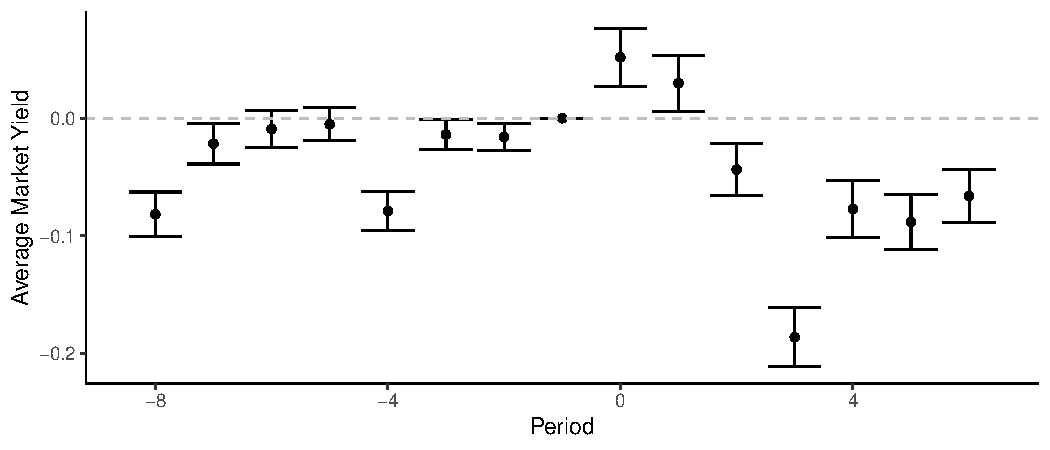
\includegraphics[width = \linewidth]{NEA_Market_Yield_Graph.pdf}
		\footnotesize{Figure plots the event study coefficients from Table \ref{tab:NEA_Market_Yield}. Base period is 2021 Quarter 2. All data from 2020 and the first quarter of 2021 is excluded, and as such, Period -1 is the fourth quarter of 2019. Standard errors clustered at the level of origin-destination pairs are reported. }
	\end{figure}
	
	\begin{figure}
		\caption{NEA Market Yield - Airport Interactions}
		\label{fig:NEA_Market_Yield_Interaction}
		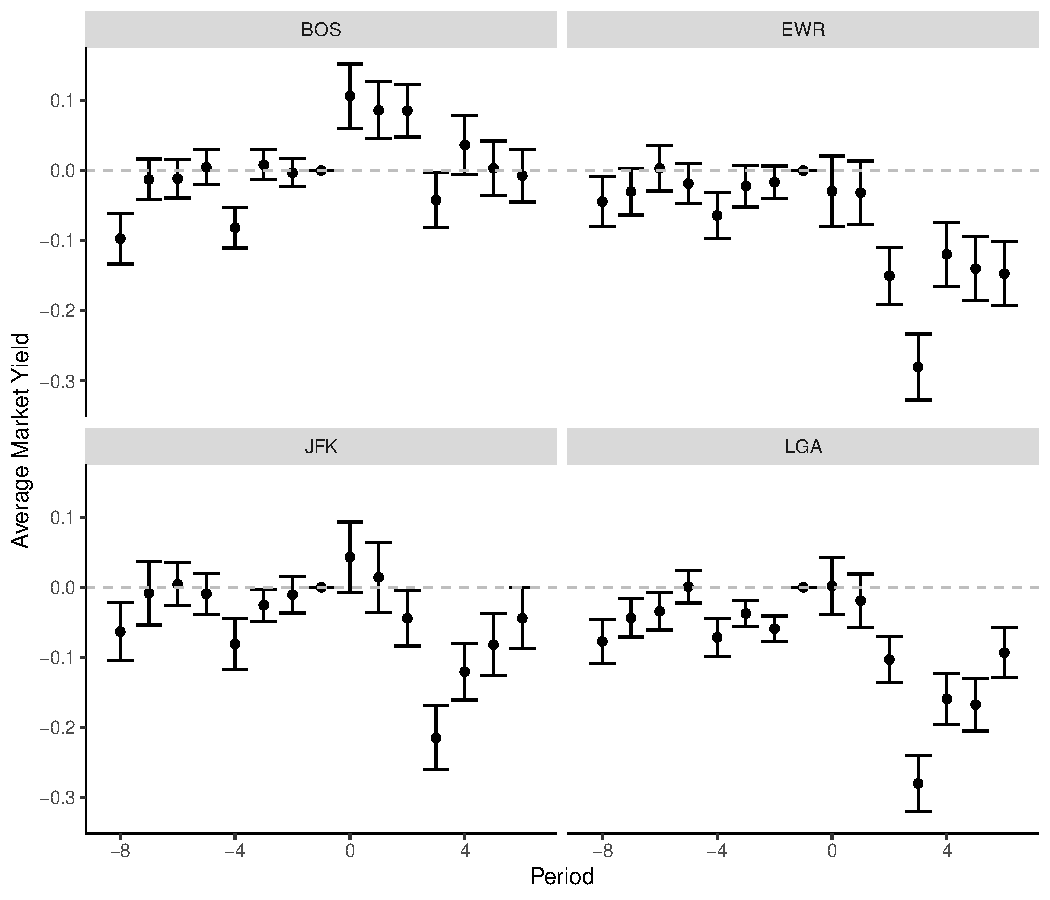
\includegraphics[width = \linewidth]{NEA_Airport_Yield_Graph}
		\footnotesize{Coefficients from a model based on the model reported in Table \ref{tab:NEA_Market_Yield} but which includes airport-time interaction terms are reported. Base period is 2021 Quarter 2. All data from 2020 and the first quarter of 2021 is excluded, and as such, Period -1 is the fourth quarter of 2019. Standard errors clustered at the level of origin-destination pairs are reported. }
	\end{figure}	
	
	\subsection{Estimation Results: JetBlue-Spirit Merger}
	
	
	\begin{table}[h]
		\caption{Elasticity Comparison Table}
		\label{tab:ElasticityComparison}
		
\begin{tabular}[t]{llll}
\toprule
Paper & Period Analyzed & Estimated Average Elasticity & Notes\\
\midrule
\addlinespace[0.3em]
\multicolumn{4}{l}{\textbf{Prior Literature}}\\
\hspace{1em}Berry and Jia (2010) & 1999 & -1.69 & \\
\hspace{1em}Berry and Jia (2010) & 2006 & -1.67 & \\
\hspace{1em}Gayle (2013) & 2006Q1 - 2006Q4 & -4.72 & \\
\hspace{1em}Ciliberto and Williams (2014) & 2006Q1 - 2008Q4 & -4.320 & \\
\hspace{1em}Ciliberto and Williams (2021) & 2012Q2 & {}[-7.281, -7.063] & Median, Exogeneous Entry Model\\
\hspace{1em}Ciliberto and Williams (2021) & 2012Q2 & {}[-4.105, -4.007] & Median, Endogeneous Entry Model\\
\hspace{1em}Turner (2022) & 2000Q3 & -2.107 & \\
\hspace{1em}Turner (2022) & 2018Q3 & -4.102 & \\
\addlinespace[0.3em]
\multicolumn{4}{l}{\textbf{New Results}}\\
\hspace{1em} & 2017Q1 - 2019Q4 & -5.591 & \\
\hspace{1em} & 2021Q2 - 2023Q2 & -5.211 & \\
\bottomrule
\end{tabular}

	\end{table}
	
	\begin{table}
		\caption{Demand Estimation}
		\label{tab:DemandEstimation_OriginalInstruments}
		
\begin{tabular}[t]{lll}
\toprule
Variable & Post-Pandemic & Pre-Pandemic\\
\midrule
\addlinespace[0.3em]
\multicolumn{3}{l}{\textbf{Linear Coefficients}}\\
\hspace{1em}Prices & -7.53*** & -2.63***\\
\hspace{1em} & (2.5) & (0.27)\\
\hspace{1em}Nonstop & -2.85** & 0.887\\
\hspace{1em} & (1.2) & (1.6)\\
\hspace{1em}Miles Flown & 7.11*** & 0.846***\\
\hspace{1em} & (1.8) & (0.099)\\
\hspace{1em}Miles Flown$^2$ & -0.749*** & -0.0817***\\
\hspace{1em} & (0.24) & (0.022)\\
\hspace{1em}Extra Miles & -2.62*** & -1.75***\\
\hspace{1em} & (0.48) & (0.078)\\
\hspace{1em}Tourism & -0.173 & 0.149***\\
\hspace{1em} & (0.12) & (0.022)\\
\addlinespace[0.3em]
\multicolumn{3}{l}{\textbf{Nonlinear Standard Deviations}}\\
\hspace{1em}Price & 0.227 & 0.675***\\
\hspace{1em} & (0.88) & (0.083)\\
\hspace{1em}Nonstop & 2.75*** & 0.716\\
\hspace{1em} & (0.56) & (2.4)\\
\addlinespace[0.3em]
\multicolumn{3}{l}{\textbf{Nesting Coefficient}}\\
\hspace{1em}Nesting Coefficient & 0.823*** & 0.823***\\
\hspace{1em} & (0.82) & (0.01)\\
\addlinespace[0.3em]
\multicolumn{3}{l}{\textbf{Summary Statistics}}\\
\hspace{1em}Period & 2017Q1-2019Q4 & 2021Q2:2023Q2\\
\hspace{1em}N Products & 284830 & 337137\\
\hspace{1em}N Markets & 85841 & 111587\\
\hspace{1em}Mean Elasticity & -47.404 & -3.557\\
\hspace{1em}Spirit Mean Elasticity & -37.28 & -2.23\\
\hspace{1em}JetBlue Mean Elasticity & -66.43 & -3.5\\
\hspace{1em}Mean Markup & 0.031 & 0.294\\
\bottomrule
\end{tabular}

		\footnotesize{$^{***}p<0.01$; $^{**}p<0.05$; $^{*}p<0.1$ Products are defined as a Carrier-Nonstop pair within an Origin-Destination-Year-Quarter market. Origin Service Ratio is the fraction of direct routes out of the originating airport operated by the carrier divided by the number of distinct direct routes out fo that airport. Extra Miles is the average additional miles flown with a connecting itinerary minus the minimum miles flown within a market.  A tourist product is one that serves the Las Vegas metropolitan statistical area or an airport in Florida.}
	\end{table}
	
	
	\FloatBarrier
	
	\subsubsection{Pre-Pandemic Period}
	
	\begin{table}
		\caption{Summary Statistics - Product Level, Pre-Pandemic}
		\label{tab:SummaryStatistics_Products_Pre}
		
\begin{tabular}[t]{lllll}
\toprule
Variable & All Firms & JetBlue & Spirit & Legacy\\
\midrule
\addlinespace[0.3em]
\multicolumn{5}{l}{\textbf{Price (100s 2017 USD)}}\\
\hspace{1em}Min & 0.34 & 0.69 & 0.35 & 0.44\\
\hspace{1em}Median & 2.39 & 2.1 & 1.19 & 2.6\\
\hspace{1em}Mean & 2.37 & 2.13 & 1.23 & 2.61\\
\hspace{1em}(SD) & (0.7) & (0.62) & (0.45) & (0.6)\\
\hspace{1em}Max & 8.11 & 7.24 & 3.85 & 8.11\\
\addlinespace[0.3em]
\multicolumn{5}{l}{\textbf{Number of Passengers}}\\
\hspace{1em}Min & 100 & 100 & 100 & 100\\
\hspace{1em}Median & 670 & 370 & 1030 & 540\\
\hspace{1em}Mean & 3897.32 & 8108.51 & 6365.64 & 3100.94\\
\hspace{1em}(SD) & (9799.72) & (14798.97) & (9315.46) & (8981.32)\\
\hspace{1em}Max & 192050 & 138880 & 66610 & 192050\\
\addlinespace[0.3em]
\multicolumn{5}{l}{\textbf{Miles Flown (Thousands)}}\\
\hspace{1em}Min & 0.15 & 0.18 & 0.18 & 0.15\\
\hspace{1em}Median & 1.26 & 1.37 & 1.46 & 1.25\\
\hspace{1em}Mean & 1.4 & 1.69 & 1.52 & 1.38\\
\hspace{1em}(SD) & (0.67) & (0.91) & (0.68) & (0.66)\\
\hspace{1em}Max & 7.57 & 3.87 & 3.52 & 3.63\\
\addlinespace[0.3em]
\multicolumn{5}{l}{\textbf{Origin Route Share (Percent)}}\\
\hspace{1em}Min & 0.54 & 0.54 & 1.23 & \vphantom{1} 1.23\\
\hspace{1em}Median & 18.92 & 7.32 & 13.91 & 14.29\\
\hspace{1em}Mean & 35.21 & 20.26 & 16.94 & 25.5\\
\hspace{1em}(SD) & (30.69) & (23.97) & (11.01) & (25.93)\\
\hspace{1em}Max & 100 & 100 & 83.33 & \vphantom{1} 100\\
\addlinespace[0.3em]
\multicolumn{5}{l}{\textbf{Destination Route Share (Percent)}}\\
\hspace{1em}Min & 0.54 & 0.54 & 1.23 & 1.23\\
\hspace{1em}Median & 19 & 7.84 & 14.05 & 14.29\\
\hspace{1em}Mean & 35.22 & 20.54 & 17.03 & 25.49\\
\hspace{1em}(SD) & (30.65) & (23.91) & (11.02) & (25.9)\\
\hspace{1em}Max & 100 & 100 & 83.33 & 100\\
\addlinespace[0.3em]
\multicolumn{5}{l}{\textbf{Extra Miles}}\\
\hspace{1em}Median & 0.04 & 0.05 & 0.04 & 0.05\\
\hspace{1em}Mean & 0.12 & 0.23 & 0.19 & 0.12\\
\hspace{1em}(SD) & (0.18) & (0.3) & (0.26) & (0.17)\\
\hspace{1em}Max & 4.98 & 1.52 & 1.46 & 1.57\\
\addlinespace[0.3em]
\multicolumn{5}{l}{\textbf{JetFuel * Market Miles}}\\
\hspace{1em}Min & 0.21 & 0.26 & 0.25 & 0.21\\
\hspace{1em}Median & 2.3 & 2.59 & 2.67 & 2.27\\
\hspace{1em}Mean & 2.56 & 3.11 & 2.81 & 2.52\\
\hspace{1em}(SD) & (2.56) & (3.11) & (2.81) & (2.52)\\
\hspace{1em}Max & 0.21 & 0.26 & 0.25 & 0.21\\
\addlinespace[0.3em]
\multicolumn{5}{l}{\textbf{Binary Variables}}\\
\hspace{1em}Share Nonstop & 0.25 & 0.39 & 0.46 & 0.17\\
\hspace{1em}Share Tourist Route & 0.26 & 0.37 & 0.42 & 0.25\\
\midrule
Observations & 337103 & 9144 & 10316 & 212051\\
\bottomrule
\end{tabular}

		\footnotesize{Data spans the period from 2017Q1 through 2019Q4. Products are defined as a one-way trip between two airports, operated as either nonstop or connecting. ``Route Shares" are the share of nonstop destinations served by the ticketing carrier out of the indicated airport as a fraction of all nonstop routes that airport has service to.}
	\end{table}
	
	\begin{table}
		\caption{Summary Statistics - Market Level, Pre-Pandemic}
		\label{tab:SummaryStatistics_Market_Pre}
		
\begin{tabular}[t]{llllll}
\toprule
 & Mean & (SD) & Minimum & Median & Maximum\\
\midrule
Number of Products & 3.52 & ( 2.11 ) & 1 & 3 & 15\\
Share Nonstop Products & 0.28 & ( 0.3 ) & 0 & 0.25 & 1\\
Market Size (Thousands) & 2788.68 & ( 2127.94 ) & 244.73 & 2154.82 & 16038\\
Customers in Market & 15012.74 & ( 28283.47 ) & 500 & 4200 & 406050\\
Direct Distance & 1.18 & ( 0.64 ) & 0.15 & 1.02 & 2.95\\
Tourist Market & 0.27 & ( 0.44 ) & 0 & 0 & 1\\
Delta Prescence & 0.72 & ( 0.45 ) & 0 & 1 & 1\\
United Presence & 0.42 & ( 0.49 ) & 0 & 0 & 1\\
American Prescence & 0.65 & ( 0.48 ) & 0 & 1 & 1\\
Southwest Prescence & 0.55 & ( 0.5 ) & 0 & 1 & 1\\
JetBlue Prescence & 0.09 & ( 0.28 ) & 0 & 0 & 1\\
Spirit Prescence & 0.09 & ( 0.28 ) & 0 & 0 & 1\\
\midrule
Observations & 87363 &  &  &  & \\
\bottomrule
\end{tabular}

		\footnotesize{Data spans the period from 2017Q1 through 2019Q4. Markets are defined as a combination of origin airport, destination airport, year, and quarter. A ``JetBlue" market is one that JetBlue operates within; a ``JetBlue-Spirit" market is one in which both firms operates within. }
	\end{table}
	
	\begin{landscape}
		\begin{table}
			\caption{Instrument Comparison Table - Pre-Pandemic}
			\label{tab:Instrument_Compare_Pre}
			
\begin{tabular}{l c c c c c c c c c}
\toprule
 & Model 1 & Model 2 & Model 3 & Model 4 & Model 5 & Model 6 & Model 7 & Model 8 & Model 9 \\
\midrule
Price                       & $-0.43^{***}$ & $-4.99^{***}$ & $-0.35^{***}$ & $-0.35^{***}$ & $-2.14^{***}$ & $-0.33^{***}$ & $-2.12^{***}$ & $-2.23^{***}$ & $-2.20^{***}$ \\
                            & $(0.00)$      & $(0.09)$      & $(0.05)$      & $(0.05)$      & $(0.04)$      & $(0.05)$      & $(0.04)$      & $(0.03)$      & $(0.03)$      \\
Nesting                     & $0.56^{***}$  & $0.44^{***}$  & $-0.11^{***}$ & $-0.11^{***}$ & $0.14^{***}$  & $-0.11^{***}$ & $0.13^{***}$  & $0.19^{***}$  & $0.19^{***}$  \\
                            & $(0.00)$      & $(0.01)$      & $(0.01)$      & $(0.01)$      & $(0.01)$      & $(0.01)$      & $(0.01)$      & $(0.00)$      & $(0.00)$      \\
\midrule
Products in Market          &               & X             & X             & X             & X             & X             & X             & X             & X             \\
Gas Instruments             &               & X             &               &               & X             &               & X             &               & X             \\
Hub Interactions            &               &               & X             & X             & X             & X             & X             & X             & X             \\
Gandhi Instruments          &               &               &               &               &               & X             & X             & X             & X             \\
Exog Interactions           &               &               &               &               &               &               &               & X             & X             \\
Price Test                  &               & 97946.457     & 91287.26      & 91287.26      & 84597.288     & 91204.891     & 84464.583     & 74792.52      & 74293.33      \\
P-Value                     &               & 0             & 0             & 0             & 0             & 0             & 0             & 0             & 0             \\
Test of Over Identification &               & N/A           & 4234.92       & 4234.92       & 7260.63       & 4368.14       & 7438.25       & 11730.66      & 12115.28      \\
p-value                     &               & N/A           & 0             & 0             & 0             & 0             & 0             & 0             & 0             \\
Mean Elasticity             & $-0.99$       & $-11.58$      & $-0.81$       & $-0.81$       & $-4.95$       & $-0.78$       & $-4.92$       & $-5.16$       & $-5.09$       \\
Median Elasticity           & $-1.01$       & $-11.76$      & $-0.82$       & $-0.82$       & $-5.03$       & $-0.79$       & $-5.00$       & $-5.24$       & $-5.17$       \\
Share Inelastic Products    & $0.49$        & $0.00$        & $0.79$        & $0.79$        & $0.00$        & $0.84$        & $0.00$        & $0.00$        & $0.00$        \\
Share JB Inelastic Products & $0.66$        & $0.00$        & $0.89$        & $0.89$        & $0.00$        & $0.92$        & $0.00$        & $0.00$        & $0.00$        \\
Share SP Inelastic Products & $1$           & $0$           & $1$           & $1$           & $0$           & $1$           & $0$           & $0$           & $0$           \\
Num. obs.                   & $307849$      & $307849$      & $307849$      & $307849$      & $307849$      & $307849$      & $307849$      & $307849$      & $307849$      \\
\bottomrule
\multicolumn{10}{l}{\scriptsize{$^{***}p<0.001$; $^{**}p<0.01$; $^{*}p<0.05$}}
\end{tabular}

			\footnotesize{Dependent variables is the difference between the estimated log-product share and the log-product share of the outside variable. Each column includes all instruments from previous columns.}
		\end{table}
	\end{landscape}
	
	
	\begin{table}
		\caption{Pre-Pandemic Demand Estimation Results}
		\label{tab:Results_PrePandemic}
		
\begin{tabular}[t]{llll}
\toprule
\addlinespace[0.3em]
\multicolumn{4}{l}{\textbf{Linear Coefficients}}\\
\hspace{1em}Prices & NonStop & Miles Flown & Miles Squared\\
\hspace{1em}-7.13** & -1.01 & 5.16** & -0.955\\
\hspace{1em}(4.3) & (2.2) & (4.5) & (0.84)\\
\hspace{1em}Origin Service Ratio & Extra Miles & Tourist & \\
\hspace{1em}0.0198 & -2.65*** & -0.304 & \\
\hspace{1em}(0.0096) & (0.66) & (0.51) & \\
\addlinespace[0.3em]
\multicolumn{4}{l}{\textbf{Nonlinear Standard Deviations}}\\
\hspace{1em} & Price & Nonstop & \\
\hspace{1em}Coefficient & 1.14*** & 2.01** & \\
\hspace{1em}SE & (0.251) & (1.07) & \\
\midrule
\addlinespace[0.3em]
\multicolumn{4}{l}{\textbf{Summary Statistics}}\\
\hspace{1em}Nesting Parameter: & 0.0881 & SE: & (0.26)\\
\hspace{1em}N Products & 337137 & N Markets & 111587\\
\hspace{1em}Mean Elasticity: & -9.93 & Mean Markup: & 0.104\\
\hspace{1em}Spirit Mean E & -6.51 & JetBlue Mean E & -10.4\\
\bottomrule
\end{tabular}

		\footnotesize{$^{***}p<0.01$; $^{**}p<0.05$; $^{*}p<0.1$ Products are defined as a Carrier-Nonstop pair within an Origin-Destination-Year-Quarter market. Origin Service Ratio is the fraction of direct routes out of the originating airport operated by the carrier divided by the number of distinct direct routes out fo that airport. Extra Miles is the average additional miles flown with a connecting itinerary minus the minimum miles flown within a market.  A tourist product is one that serves the Las Vegas metropolitan statistical area or an airport in Florida.}
	\end{table}
	
	\begin{table}
		\caption{Pre-Pandemic Merger Simulation (Basic)}
		\label{tab:Simulation_Pre_Basic}
		
\begin{tabular}[t]{llllll}
\toprule
\multicolumn{1}{c}{ } & \multicolumn{3}{c}{Obseved Sample} & \multicolumn{2}{c}{Basic Merger} \\
\cmidrule(l{3pt}r{3pt}){2-4} \cmidrule(l{3pt}r{3pt}){5-6}
\multicolumn{1}{c}{Variable} & \multicolumn{1}{c}{Spirit} & \multicolumn{1}{c}{JetBlue} & \multicolumn{1}{c}{Other} & \multicolumn{1}{c}{Merged} & \multicolumn{1}{c}{Other} \\
\cmidrule(l{3pt}r{3pt}){1-1} \cmidrule(l{3pt}r{3pt}){2-2} \cmidrule(l{3pt}r{3pt}){3-3} \cmidrule(l{3pt}r{3pt}){4-4} \cmidrule(l{3pt}r{3pt}){5-5} \cmidrule(l{3pt}r{3pt}){6-6}
\addlinespace[0.3em]
\multicolumn{6}{l}{\textbf{Passengers}}\\
\hspace{1em}Minimum & 100 & 100 & 740 & 210 & 741\\
\hspace{1em}Average & 11300 & 15600 & 53600 & 26200 & 53600\\
\hspace{1em}Maximum & 67000 & 89700 & 315000 & 129000 & 315000\\
\addlinespace[0.3em]
\multicolumn{6}{l}{\textbf{Market Share}}\\
\hspace{1em}Minimum & 9.36e-06 & 6.24e-06 & 4.65e-05 & 2.18e-05 & 4.65e-05\\
\hspace{1em}Average & 0.00252 & 0.00373 & 0.0103 & 0.00605 & 0.0104\\
\hspace{1em}Maximum & 0.0202 & 0.0419 & 0.0447 & 0.0515 & 0.0447\\
\addlinespace[0.3em]
\multicolumn{6}{l}{\textbf{Prices}}\\
\hspace{1em}Minimum & 0.463 & 0.732 & 0.885 & 0.549 & 0.885\\
\hspace{1em}Average & 1.07 & 2.01 & 2.09 & 1.49 & 2.09\\
\hspace{1em}Maximum & 2.82 & 4.76 & 3.42 & 3.18 & 3.42\\
\addlinespace[0.3em]
\multicolumn{6}{l}{\textbf{Marginal Cost}}\\
\hspace{1em}Minimum & 0.153 & 0.411 & 0.543 & 0.233 & 0.543\\
\hspace{1em}Average & 0.73 & 1.61 & 1.68 & 1.12 & 1.68\\
\hspace{1em}Maximum & 2.42 & 4.25 & 2.91 & 2.71 & 2.91\\
\addlinespace[0.3em]
\multicolumn{6}{l}{\textbf{Miles Flown}}\\
\hspace{1em}Minimum & 0.319 & 0.319 & 0.319 & 0.319 & 0.319\\
\hspace{1em}Average & 1.58 & 1.65 & 1.48 & 1.54 & 1.48\\
\hspace{1em}Maximum & 3.52 & 3.72 & 2.89 & 3.52 & 2.89\\
\addlinespace[0.3em]
\multicolumn{6}{l}{\textbf{Origin Service Ratio}}\\
\hspace{1em}Minimum & 1.23 & 0.541 & 6.72 & 0.8 & 6.72\\
\hspace{1em}Average & 17.5 & 17.2 & 47.3 & 19.8 & 47.3\\
\hspace{1em}Maximum & 44.7 & 71.2 & 95.7 & 70.6 & 95.7\\
\midrule
Number of Markets & 1533 & 1533 & 1533 & 1533 & 1533\\
\bottomrule
\end{tabular}

		\footnotesize{Merger simulation results for the "basic" merger simulation are reported. Only markets with both firms included are present in these estimates. This simulation assumes that product offerings do not change following the merger, and serves to capture effects resulting from the internalization of the pricing externality following the merger. Cells are market average product characteristics across firms within a category, weighted by product shares.}
	\end{table}
	
	\begin{landscape}
		\begin{table}
			\caption{Pre-Pandemic Merger Simulation, Joint Markets}
			\label{tab:Simulation_Pre}
			
\begin{tabular}[t]{llllll}
\toprule
 & Mean & (SD) & Minimum & Median & Maximum\\
\midrule
\addlinespace[0.3em]
\multicolumn{6}{l}{\textbf{Prices}}\\
\hspace{1em}Best Case & 2.12 & (0.67) & 0.51 & 2.07 & 5.11\\
\hspace{1em}Average Case & 2.16 & (0.64) & 0.51 & 2.11 & 5.11\\
\hspace{1em}Worst Case & 2.21 & (0.64) & 0.51 & 2.14 & 5.11\\
\addlinespace[0.3em]
\multicolumn{6}{l}{\textbf{Price Change}}\\
\hspace{1em}Best Case & -0.03 & (0.25) & -3.04 & 0.05 & 0.21\\
\hspace{1em}Average Case & 0.01 & (0.14) & -1.47 & 0.05 & 1.11\\
\hspace{1em}Worst Case & 0.06 & (0.11) & -0.74 & 0.05 & 2.18\\
\addlinespace[0.3em]
\multicolumn{6}{l}{\textbf{Within Market Shares}}\\
\hspace{1em}Best Case & 0.14 & (0.21) & 0 & 0.04 & 0.97\\
\hspace{1em}Average Case & 0.12 & (0.17) & 0 & 0.04 & 0.95\\
\hspace{1em}Worst Case & 0.11 & (0.16) & 0 & 0.03 & 0.95\\
\addlinespace[0.3em]
\multicolumn{6}{l}{\textbf{Within Market Shares Change}}\\
\hspace{1em}Best Case & 0 & (0.1) & -0.55 & 0 & 0.63\\
\hspace{1em}Average Case & -0.02 & (0.1) & -0.67 & 0 & 0.33\\
\hspace{1em}Average Case & -0.03 & (0.12) & -0.83 & 0 & 0.33\\
\bottomrule
\end{tabular}

			\footnotesize{Merger simulation results for the post-pandemic sample are reported. The "Other" category consists of the average other product in each market, constructed by a weighted average on the basis of estimated passengers. Then, this is averaged across all markets. The "Low-Cost Merger" ("Mean Cost Merger") ["High Cost Merger"] refers to the counterfactual scenario where the merged firm has the lowest (average) [highest] marginal cost of the two merged firms for each product.}
		\end{table}
	\end{landscape}

	
	\begin{figure}
		\caption{Change in Lowest Market Fare, Pre-Pandemic}
		\label{fig:LowestMarketChange_Pre}
		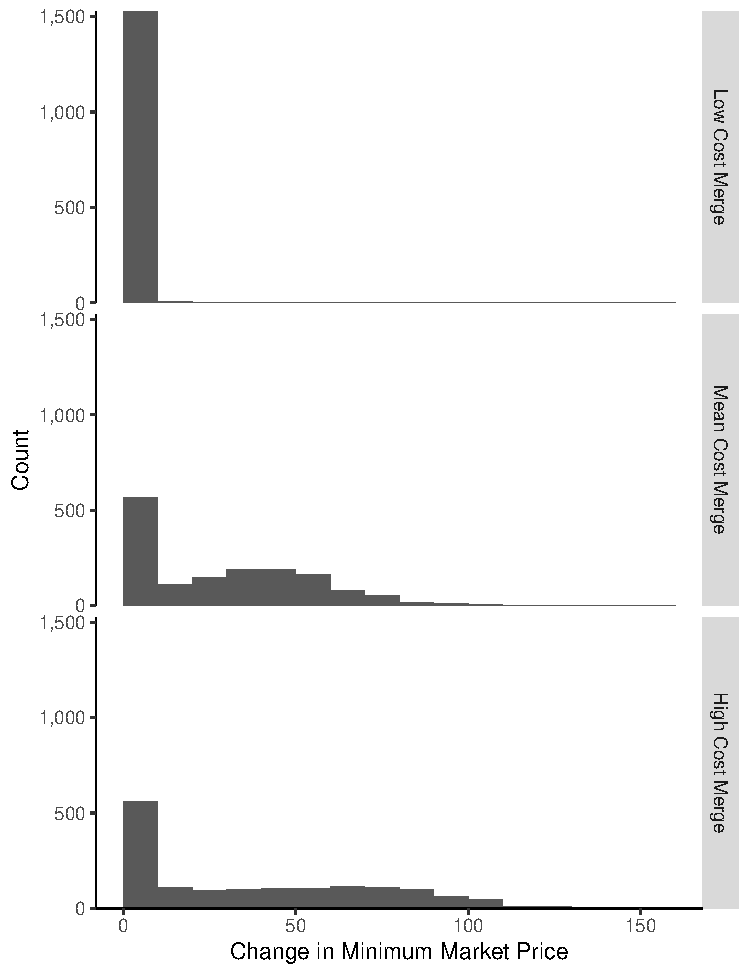
\includegraphics[width = \linewidth]{PrePandemic_Merger_Change_MinimumFare}
		\footnotesize{Plotted change in the price of the minimum fare within a market following the simulated merger, for markets included in the post-pandemic sample. The "Low-Cost Merger" ("Mean Cost Merger") ["High Cost Merger"] refers to the counterfactual scenario where the merged firm has the lowest (average) [highest] marginal cost of the two merged firms for each product. Each histogram bar covers a range of \$10 increments.}
	\end{figure}
	
	\FloatBarrier
	\subsubsection{Post-Pandemic Period}
		\begin{table}
		\caption{Summary Statistics - Product Level, Post-Pandemic}
		\label{tab:SummaryStatistics_Products_Post}
		
\begin{tabular}[t]{lllll}
\toprule
Variable & All Firms & JetBlue & Spirit & Legacy\\
\midrule
\addlinespace[0.3em]
\multicolumn{5}{l}{\textbf{Price (100s 2017 USD)}}\\
\hspace{1em}Min & 0.24 & 0.61 & 0.29 & 0.55\\
\hspace{1em}Median & 2.13 & 1.93 & 1.19 & 2.4\\
\hspace{1em}Mean & 2.17 & 2 & 1.24 & 2.46\\
\hspace{1em}(SD) & (0.75) & (0.64) & (0.45) & (0.67)\\
\hspace{1em}Max & 6.52 & 4.96 & 4.1 & 6.52\\
\addlinespace[0.3em]
\multicolumn{5}{l}{\textbf{Number of Passengers}}\\
\hspace{1em}Min & 100 & 100 & 100 & 100\\
\hspace{1em}Median & 610 & 670 & 670 & 520\\
\hspace{1em}Mean & 3302.07 & 6893.11 & 5023.04 & 2803.36\\
\hspace{1em}(SD) & (8387.84) & (13383.88) & (8608.73) & (8056.87)\\
\hspace{1em}Max & 144930 & 115000 & 68030 & 140870\\
\addlinespace[0.3em]
\multicolumn{5}{l}{\textbf{Miles Flown (Thousands)}}\\
\hspace{1em}Min & 0.15 & 0.18 & 0.18 & 0.15\\
\hspace{1em}Median & 1.27 & 1.5 & 1.49 & 1.28\\
\hspace{1em}Mean & 1.41 & 1.75 & 1.54 & 1.41\\
\hspace{1em}(SD) & (0.67) & (0.95) & (0.67) & (0.66)\\
\hspace{1em}Max & 3.86 & 3.79 & 3.58 & 3.61\\
\addlinespace[0.3em]
\multicolumn{5}{l}{\textbf{Origin Route Share (Percent)}}\\
\hspace{1em}Min & 0.53 & 0.9 & 0.9 & 0.99\\
\hspace{1em}Median & 18.18 & 10.87 & 11.32 & 12.77\\
\hspace{1em}Mean & 34.11 & 25.46 & 14.25 & 23.67\\
\hspace{1em}(SD) & (30.59) & (29.02) & (10.65) & (25.48)\\
\hspace{1em}Max & 100 & 100 & 47.37 & \vphantom{1} 100\\
\addlinespace[0.3em]
\multicolumn{5}{l}{\textbf{Destination Route Share (Percent)}}\\
\hspace{1em}Min & 0 & 0.9 & 0.9 & 0.99\\
\hspace{1em}Median & 18.18 & 11.36 & 11.39 & 12.77\\
\hspace{1em}Mean & 34.13 & 25.65 & 14.36 & 23.69\\
\hspace{1em}(SD) & (30.58) & (28.95) & (10.7) & (25.5)\\
\hspace{1em}Max & 100 & 100 & 47.37 & 100\\
\addlinespace[0.3em]
\multicolumn{5}{l}{\textbf{Extra Miles}}\\
\hspace{1em}Median & 0.05 & 0 & 0.07 & 0.07\\
\hspace{1em}Mean & 0.13 & 0.25 & 0.21 & 0.13\\
\hspace{1em}(SD) & (0.19) & (0.36) & (0.28) & (0.17)\\
\hspace{1em}Max & 1.83 & 1.52 & 1.41 & 1.5\\
\addlinespace[0.3em]
\multicolumn{5}{l}{\textbf{JetFuel * Market Miles}}\\
\hspace{1em}Min & 0.27 & 0.32 & 0.31 & 0.27\\
\hspace{1em}Median & 3.43 & 4.25 & 3.92 & 3.46\\
\hspace{1em}Mean & 3.86 & 4.97 & 4.26 & 3.88\\
\hspace{1em}(SD) & (3.86) & (4.97) & (4.26) & (3.88)\\
\hspace{1em}Max & 0.27 & 0.32 & 0.31 & 0.27\\
\addlinespace[0.3em]
\multicolumn{5}{l}{\textbf{Binary Variables}}\\
\hspace{1em}Share Nonstop & 0.25 & 0.5 & 0.35 & 0.17\\
\hspace{1em}Share Tourist Route & 0.28 & 0.42 & 0.42 & 0.26\\
\midrule
Observations & 284802 & 7350 & 11463 & 167160\\
\bottomrule
\end{tabular}

		\footnotesize{Data spans the period from 2021Q2 through 2023Q2. Products are defined as a one-way trip between two airports, operated as either nonstop or connecting. ``Route Shares" are the share of nonstop destinations served by the ticketing carrier out of the indicated airport as a fraction of all nonstop routes that airport has service to. }
	\end{table}
	
	\begin{table}
		\caption{Summary Statistics - Market Level, Post-Pandemic}
		\label{tab:SummaryStatistics_Market_Post}
		
\begin{tabular}[t]{llllll}
\toprule
 & Mean & (SD) & Minimum & Median & Maximum\\
\midrule
Number of Products & 3.79 & (2.16) & 1 & 3 & 14\\
Share Nonstop Products & 0.27 & (0.31) & 0 & 0.22 & 1\\
Market Size (Thousands) & 2795.51 & (2142.87) & 223.81 & 2161.62 & 16141.64\\
Customers in Market & 13422.5 & (25089.6) & 500 & 3880 & 317410\\
Direct Distance & 1.19 & (0.64) & 0.15 & 1.04 & 2.96\\
Tourist Market & 0.27 & (0.44) & 0 & 0 & 1\\
Delta Prescence & 0.72 & (0.45) & 0 & 1 & 1\\
United Presence & 0.44 & (0.5) & 0 & 0 & 1\\
American Prescence & 0.71 & (0.46) & 0 & 1 & 1\\
Southwest Prescence & 0.66 & (0.47) & 0 & 1 & 1\\
JetBlue Prescence & 0.08 & (0.28) & 0 & 0 & 1\\
Spirit Prescence & 0.13 & (0.34) & 0 & 0 & 1\\
\midrule
Observations & 70016 &  &  &  & \\
\bottomrule
\end{tabular}

		\footnotesize{Data spans the period from 2021Q2 through 2023Q2. Markets are defined as a combination of origin airport, destination airport, year, and quarter. A ``JetBlue" market is one that JetBlue operates within; a ``JetBlue-Spirit" market is one in which both firms operates within. }
	\end{table}
	
	\begin{landscape}
		\begin{table}
			\caption{Instrument Comparison Table - Post-Pandemic}
			\label{tab:Instrument_Compare}
			
\begin{tabular}{l c c c c c c c c c}
\toprule
 & Model 1 & Model 2 & Model 3 & Model 4 & Model 5 & Model 6 & Model 7 & Model 8 & Model 9 \\
\midrule
Price                       & $-0.24^{***}$ & $-0.06$       & $1.50^{***}$  & $1.50^{***}$  & $0.01$        & $1.28^{***}$  & $-0.00$       & $-2.46^{***}$ & $-0.63^{***}$ \\
                            & $(0.00)$      & $(0.03)$      & $(0.16)$      & $(0.16)$      & $(0.03)$      & $(0.15)$      & $(0.03)$      & $(0.07)$      & $(0.03)$      \\
Nesting                     & $0.54^{***}$  & $-0.11^{***}$ & $-0.26^{***}$ & $-0.26^{***}$ & $-0.11^{***}$ & $-0.24^{***}$ & $-0.11^{***}$ & $0.15^{***}$  & $0.01^{**}$   \\
                            & $(0.00)$      & $(0.00)$      & $(0.01)$      & $(0.01)$      & $(0.00)$      & $(0.01)$      & $(0.00)$      & $(0.01)$      & $(0.00)$      \\
\midrule
Products in Market          &               & X             & X             & X             & X             & X             & X             & X             & X             \\
Gas Instruments             &               & X             &               &               & X             &               & X             &               & X             \\
Hub Interactions            &               &               & X             & X             & X             & X             & X             & X             & X             \\
Gandhi Instruments          &               &               &               &               &               & X             & X             & X             & X             \\
Exog Interactions           &               &               &               &               &               &               &               & X             & X             \\
Price Test                  &               & 77288.49      & 81853.459     & 81853.459     & 76910.107     & 81743.441     & 76883.509     & 66904.122     & 64536.553     \\
p-Value                     &               & 0             & 0             & 0             & 0             & 0             & 0             & 0             & 0             \\
Test of Over Identification &               & N/A           & 1269.2        & 1269.2        & 4165.87       & 1453.45       & 4271.75       & 7094.09       & 11604.74      \\
p-value                     &               & N/A           & 0             & 0             & 0             & 0             & 0             & 0             & 0             \\
R-Squared                   & $0.65$        & $0.34$        & $0.02$        & $0.02$        & $0.34$        & $0.09$        & $0.34$        & $0.16$        & $0.42$        \\
Adj. R-Squared              & $0.65$        & $0.34$        & $0.02$        & $0.02$        & $0.34$        & $0.08$        & $0.34$        & $0.16$        & $0.42$        \\
Mean Elasticity             & $-0.50$       & $-0.14$       & $3.19$        & $3.19$        & $0.02$        & $2.72$        & $0.00$        & $-5.22$       & $-1.34$       \\
Median Elasticity           & $-0.50$       & $-0.13$       & $3.14$        & $3.14$        & $0.02$        & $2.69$        & $0.00$        & $-5.15$       & $-1.33$       \\
Share Inelastic Products    & $1.00$        & $1.00$        & $0.02$        & $0.02$        & $1.00$        & $0.04$        & $1.00$        & $0.00$        & $0.23$        \\
Share JB Inelastic Products & $1.00$        & $1.00$        & $0.00$        & $0.00$        & $1.00$        & $0.01$        & $1.00$        & $0.00$        & $0.30$        \\
Share SP Inelastic Products & $1.00$        & $1.00$        & $0.11$        & $0.11$        & $1.00$        & $0.22$        & $1.00$        & $0.00$        & $0.84$        \\
Num. obs.                   & $265196$      & $265196$      & $265196$      & $265196$      & $265196$      & $265196$      & $265196$      & $265196$      & $265196$      \\
\bottomrule
\multicolumn{10}{l}{\scriptsize{$^{***}p<0.001$; $^{**}p<0.01$; $^{*}p<0.05$}}
\end{tabular}

		\end{table}
	\end{landscape}
	
\begin{table}
	\caption{Post-Pandemic Merger Simulation (Basic)}
	\label{tab:Simulation_Post_Basic}
	
\begin{tabular}[t]{llllll}
\toprule
\multicolumn{1}{c}{ } & \multicolumn{3}{c}{Obseved Sample} & \multicolumn{2}{c}{Basic Merger} \\
\cmidrule(l{3pt}r{3pt}){2-4} \cmidrule(l{3pt}r{3pt}){5-6}
\multicolumn{1}{c}{Variable} & \multicolumn{1}{c}{Spirit} & \multicolumn{1}{c}{JetBlue} & \multicolumn{1}{c}{Other} & \multicolumn{1}{c}{Merged} & \multicolumn{1}{c}{Other} \\
\cmidrule(l{3pt}r{3pt}){1-1} \cmidrule(l{3pt}r{3pt}){2-2} \cmidrule(l{3pt}r{3pt}){3-3} \cmidrule(l{3pt}r{3pt}){4-4} \cmidrule(l{3pt}r{3pt}){5-5} \cmidrule(l{3pt}r{3pt}){6-6}
\addlinespace[0.3em]
\multicolumn{6}{l}{\textbf{Passengers}}\\
\hspace{1em}Minimum & 100 & 100 & 1890 & 100 & 1890\\
\hspace{1em}Average & 11000 & 11500 & 51400 & 21100 & 51500\\
\hspace{1em}Maximum & 69000 & 87200 & 249000 & 116000 & 249000\\
\addlinespace[0.3em]
\multicolumn{6}{l}{\textbf{Market Share}}\\
\hspace{1em}Minimum & 8.01e-06 & 6.24e-06 & 0.000493 & 7.55e-06 & 0.000493\\
\hspace{1em}Average & 0.0023 & 0.0026 & 0.00974 & 0.00459 & 0.00975\\
\hspace{1em}Maximum & 0.0166 & 0.0346 & 0.0457 & 0.0376 & 0.0457\\
\addlinespace[0.3em]
\multicolumn{6}{l}{\textbf{Prices}}\\
\hspace{1em}Minimum & 0.61 & 0.631 & 0.765 & 0.662 & 0.765\\
\hspace{1em}Average & 1.54 & 1.89 & 2.1 & 1.71 & 2.1\\
\hspace{1em}Maximum & 5.26 & 4.42 & 4.01 & 5.21 & 4.01\\
\addlinespace[0.3em]
\multicolumn{6}{l}{\textbf{Marginal Cost}}\\
\hspace{1em}Minimum & 0.338 & 0.358 & 0.479 & 0.382 & 0.479\\
\hspace{1em}Average & 1.22 & 1.55 & 1.74 & 1.38 & 1.74\\
\hspace{1em}Maximum & 4.78 & 3.96 & 3.57 & 4.73 & 3.57\\
\addlinespace[0.3em]
\multicolumn{6}{l}{\textbf{Miles Flown}}\\
\hspace{1em}Minimum & 0.2 & 0.2 & 0.2 & 0.2 & 0.2\\
\hspace{1em}Average & 1.71 & 1.79 & 1.56 & 1.7 & 1.56\\
\hspace{1em}Maximum & 4.83 & 3.75 & 2.88 & 4.6 & 2.88\\
\addlinespace[0.3em]
\multicolumn{6}{l}{\textbf{Origin Service Ratio}}\\
\hspace{1em}Minimum & 0.901 & 0.901 & 6.17 & 0.901 & 6.17\\
\hspace{1em}Average & 17.5 & 19.7 & 44.5 & 21 & 44.5\\
\hspace{1em}Maximum & 41.2 & 79.1 & 97.5 & 78.7 & 97.5\\
\midrule
Number of Markets & 1554 & 1554 & 1554 & 1554 & 1554\\
\bottomrule
\end{tabular}

	\footnotesize{Merger simulation results for the "basic" merger simulation are reported. This simulation assumes that product offerings do not change following the merger, and serves to capture effects resulting from the internalization of the pricing externality following the merger. Cells are market average product characteristics across firms within a category, weighted by product shares.}
\end{table}
	
	\begin{landscape}
		\begin{table}
			\caption{Post-Pandemic Merger Simulation, Joint Markets}
			\label{tab:Simulation_Post}
			
\begin{tabular}[t]{lllllll}
\toprule
 & N & Mean & (SD) & Minimum & Median & Maximum\\
\midrule
\addlinespace[0.3em]
\multicolumn{7}{l}{\textbf{Pre-Pandemic}}\\
\addlinespace[0.3em]
\multicolumn{7}{l}{\textbf{Product Prices (100s, 2017 USD)}}\\
\hspace{1em}\hspace{1em}Observed & 12074 & 2.04 & (0.69) & 0.47 & 1.98 & 4.91\\
\hspace{1em}\hspace{1em}Best Case & 10106 & 2.08 & (0.66) & 0.46 & 2.02 & 5.08\\
\hspace{1em}\hspace{1em}Average Case & 10106 & 2.12 & (0.64) & 0.46 & 2.06 & 5.14\\
\hspace{1em}\hspace{1em}Worst Case & 10106 & 2.16 & (0.64) & 0.48 & 2.09 & 5.13\\
\addlinespace[0.3em]
\multicolumn{7}{l}{\textbf{Market Average Price}}\\
\hspace{1em}\hspace{1em}Observed & 1418 & 2.01 & (0.43) & 0.93 & 1.95 & \vphantom{1} 3.1\\
\hspace{1em}\hspace{1em}Best Case & 1418 & 1.73 & (0.6) & 0.81 & 1.55 & \vphantom{1} 3.44\\
\hspace{1em}\hspace{1em}Average Case & 1418 & 2 & (0.51) & 1.01 & 1.92 & \vphantom{1} 3.38\\
\hspace{1em}\hspace{1em}Worst Case & 1418 & 2.01 & (0.5) & 1 & 1.92 & \vphantom{1} 3.5\\
\addlinespace[0.3em]
\multicolumn{7}{l}{\textbf{\% Change Average Price}}\\
\hspace{1em}\hspace{1em}Best Case & 1418 & -15.13 & (16.83) & -53.06 & -16.77 & 31.42\\
\hspace{1em}\hspace{1em}Average Case & 1418 & -0.7 & (10.36) & -38.87 & -0.19 & 39.57\\
\hspace{1em}\hspace{1em}Worst Case & 1418 & 0.18 & (10.27) & -34.26 & 0.61 & 37.41\\
\addlinespace[0.3em]
\multicolumn{7}{l}{\textbf{Median Price}}\\
\hspace{1em}\hspace{1em}Observed & 1418 & 2.01 & (0.43) & 0.93 & 1.95 & 3.1\\
\hspace{1em}\hspace{1em}Best Case & 1418 & 1.73 & (0.6) & 0.81 & 1.55 & 3.44\\
\hspace{1em}\hspace{1em}Average Case & 1418 & 2 & (0.51) & 1.01 & 1.92 & 3.38\\
\hspace{1em}\hspace{1em}Worst Case & 1418 & 2.01 & (0.5) & 1 & 1.92 & 3.5\\
\midrule
\addlinespace[0.3em]
\multicolumn{7}{l}{\textbf{Post-Pandemic}}\\
\addlinespace[0.3em]
\multicolumn{7}{l}{\textbf{Product Prices  (100s, 2017 USD)}}\\
\hspace{1em}\hspace{1em}Observed & 13650 & 1.96 & (0.78) & 0.35 & 1.89 & 5.25\\
\hspace{1em}\hspace{1em}Best Case & 11496 & 2.01 & (0.77) & 0.4 & 1.94 & 5.34\\
\hspace{1em}\hspace{1em}Average Case & 11496 & 2.05 & (0.74) & 0.4 & 1.99 & 5.33\\
\hspace{1em}\hspace{1em}Worst Case & 11496 & 2.1 & (0.74) & 0.41 & 2.04 & 5.33\\
\addlinespace[0.3em]
\multicolumn{7}{l}{\textbf{Market Average Price}}\\
\hspace{1em}\hspace{1em}Observed & 1554 & 1.95 & (0.55) & 0.65 & 1.89 & \vphantom{1} 3.57\\
\hspace{1em}\hspace{1em}Best Case & 1554 & 1.71 & (0.68) & 0.61 & 1.68 & \vphantom{1} 3.67\\
\hspace{1em}\hspace{1em}Average Case & 1554 & 2.04 & (0.64) & 0.76 & 1.95 & \vphantom{1} 3.85\\
\hspace{1em}Worst Case & 1554 & 2.06 & (0.64) & 0.76 & 1.96 & \vphantom{1} 3.93\\
\addlinespace[0.3em]
\multicolumn{7}{l}{\textbf{\% Change Average Price}}\\
\hspace{1em}Best Case & 1554 & -13.67 & (18.18) & -59.32 & -10.99 & 39.39\\
\hspace{1em}Average Case & 1554 & 4.21 & (9.96) & -32.12 & 4.07 & 49.1\\
\hspace{1em}Worst Case & 1554 & 5.38 & (10) & -33.29 & 5.03 & 50.4\\
\addlinespace[0.3em]
\multicolumn{7}{l}{\textbf{Median Price}}\\
\hspace{1em}Observed & 1554 & 1.95 & (0.55) & 0.65 & 1.89 & 3.57\\
\hspace{1em}Best Case & 1554 & 1.71 & (0.68) & 0.61 & 1.68 & 3.67\\
\hspace{1em}Average Case & 1554 & 2.04 & (0.64) & 0.76 & 1.95 & 3.85\\
\hspace{1em}Worst Case & 1554 & 2.06 & (0.64) & 0.76 & 1.96 & 3.93\\
\bottomrule
\end{tabular}

			\footnotesize{Merger simulation results for the post-pandemic sample are reported. The "Other" category consists of the average other product in each market, constructed by a weighted average on the basis of estimated passengers. Then, this is averaged across all markets. The "Low-Cost Merger" ("Mean Cost Merger") ["High Cost Merger"] refers to the counterfactual scenario where the merged firm has the lowest (average) [highest] marginal cost of the two merged firms for each product.}
		\end{table}
	\end{landscape}

	\begin{figure}
		\caption{Change in Lowest Market Fare, Post-Pandemic}
		\label{fig:LowestMarketChange_Post}
		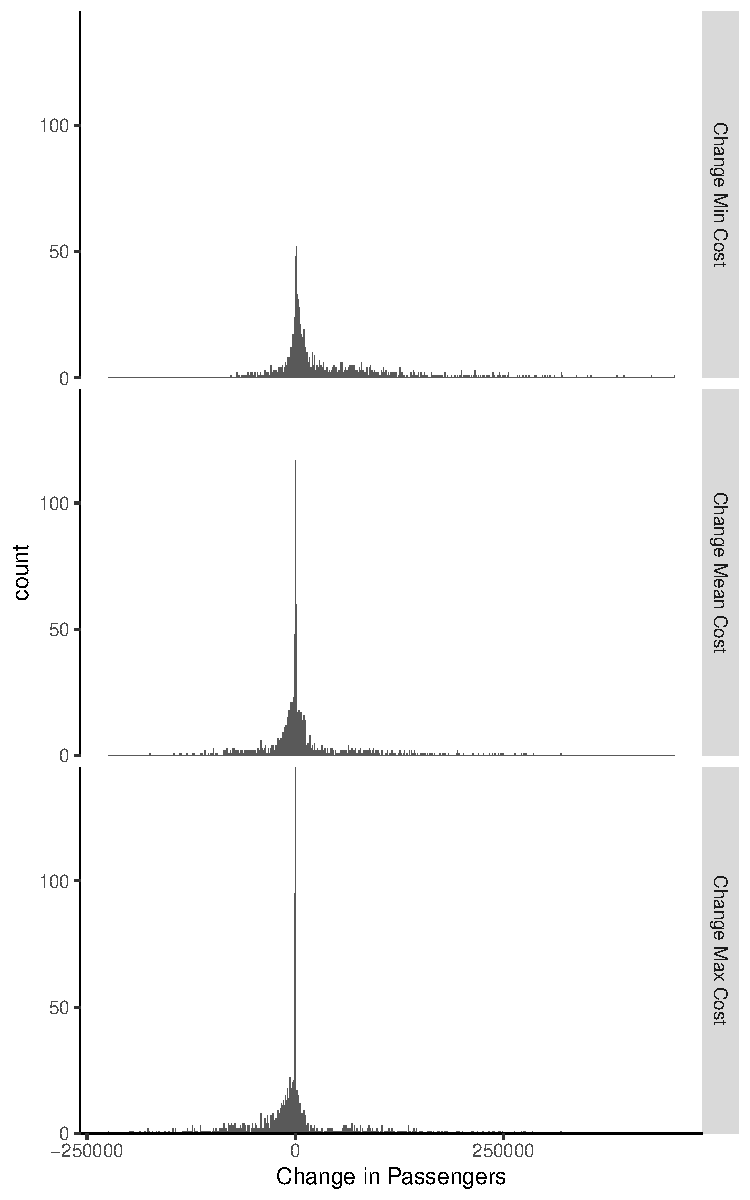
\includegraphics[width = \linewidth]{Merger_Change_MinimumFare}
		\footnotesize{Plotted change in the price of the minimum fare within a market following the simulated merger, for markets included in the post-pandemic sample. The "Low-Cost Merger" ("Mean Cost Merger") ["High Cost Merger"] refers to the counterfactual scenario where the merged firm has the lowest (average) [highest] marginal cost of the two merged firms for each product. Each histogram bar covers a range of \$10 increments.}
	\end{figure}
	
	
	\FloatBarrier
	
	\subsection{Merger Comment Processing Figures and Tables}
	\label{sec:NaturalLanguage_Figs}
	\begin{figure}[h]
		\caption{Timeline of Submitted Comments}
		\label{fig:CommentTimeline}
		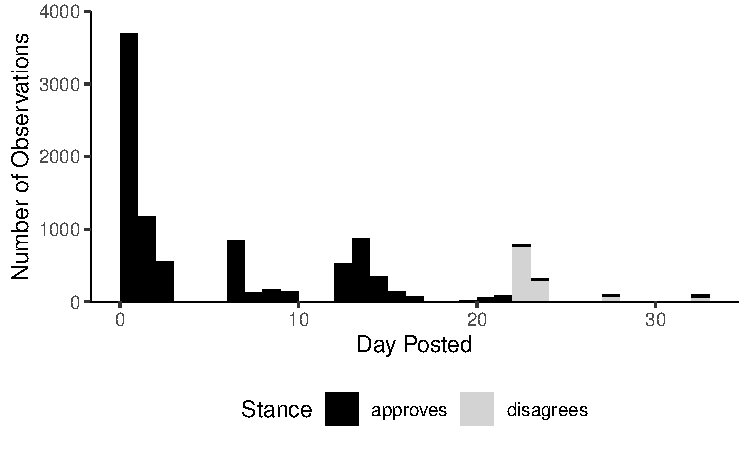
\includegraphics{stance_submission_timeline}
		\begin{minipage}{\textwidth} 
			{\footnotesize Data is sourced from the Department of Transportation regulatory filing regarding the JetBlue-Spirit merger  (DOT-OST-2023-0024). Comments have the stance with the highest probability assigned to them.} 
		\end{minipage}
	\end{figure}
	
	\begin{table}[h]
		\caption{Stance Detection Summary Statistics}
		\label{tab:Stance_Summary}
		
\begin{tabular}[t]{llllll}
\toprule
 & Mean & (SD) & Minimum & Median & Maximum\\
\midrule
\addlinespace[0.3em]
\multicolumn{6}{l}{\textbf{All Comments}}\\
\hspace{1em}P(Approves) & 0.89 & (0.31) & 0 & 1 & 1\\
\hspace{1em}Approving Comment P(Approves) & 1 & (0.02) & 0.51 & 1 & 1\\
\hspace{1em}Disapproving Comment P(Approves) & 0.01 & (0.04) & 0 & 0 & 0.49\\
\hspace{1em}New York Comment & 0.14 & (0.35) & 0 & 0 & 1\\
\hspace{1em}Florida Comment & 0.35 & (0.48) & 0 & 0 & 1\\
\hspace{1em}Massachusetts Comment & 0.05 & (0.22) & 0 & 0 & 1\\
\hspace{1em}Puerto Rico Comment & 0.01 & (0.12) & 0 & 0 & 1\\
\midrule
\hspace{1em}Observations & 10185 &  &  &  & \\
\midrule
\addlinespace[0.3em]
\multicolumn{6}{l}{\textbf{Unique Comments}}\\
\hspace{1em}P(Approves) & 0.13 & (0.32) & 0 & 0 & 1\\
\hspace{1em}Approving Comment P(Approves) & 0.98 & (0.08) & 0.51 & 1 & 1\\
\hspace{1em}Disapproving Comment P(Approves) & 0.01 & (0.06) & 0 & 0 & 0.49\\
\hspace{1em}New York Comment & 0.06 & (0.24) & 0 & 0 & 1\\
\hspace{1em}Florida Comment & 0.07 & (0.26) & 0 & 0 & 1\\
\hspace{1em}Massachusetts Comment & 0.03 & (0.18) & 0 & 0 & 1\\
\hspace{1em}Puerto Rico Comment & 0 & (0) & 0 & 0 & 0\\
\midrule
\hspace{1em}Observations & 701 &  &  &  & \\
\midrule
\bottomrule
\end{tabular}

		\begin{minipage}{\textwidth} 
			{\footnotesize Data is sourced from the Department of Transportation regulatory filing regarding the JetBlue-Spirit merger  (DOT-OST-2023-0024). Comments have the stance with the highest probability assigned to them. This is the ``Stance Probability." Similarly, ``Sentiment Assigned Probability" is the sentiment with the highest  probability assigned to a comment by the language model. Comment length is in characters.} 
		\end{minipage}
	\end{table}
	
	\begin{figure}
		\caption{Probability Comments Approve}
		\label{fig:ProbabilityApprove}
		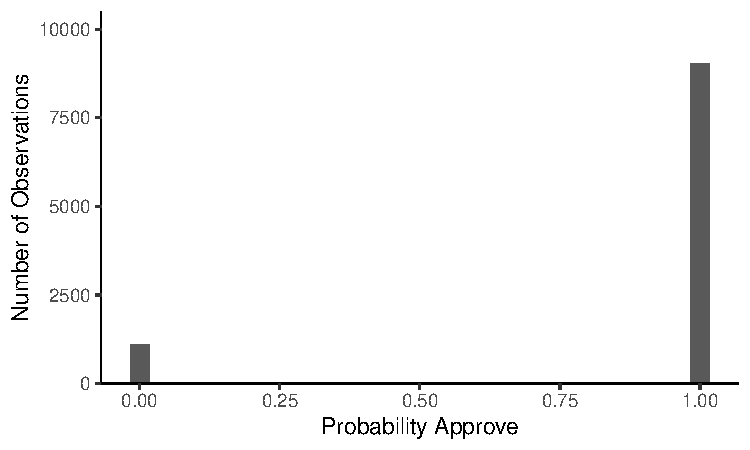
\includegraphics{05.Figures/stance_strength_graph}
		\begin{minipage}{\textwidth} 
			{\footnotesize Data is sourced from the Department of Transportation regulatory filing regarding the JetBlue-Spirit merger (DOT-OST-2023-0024). ``Probability Approve" is the probability that a comment approves of the merger.} 
		\end{minipage}
	\end{figure}
	
	\begin{figure}
		\caption{Probability Comment Approves - Unique Comments Only}
		\label{fig:ProbabilityApprove_Unique}
		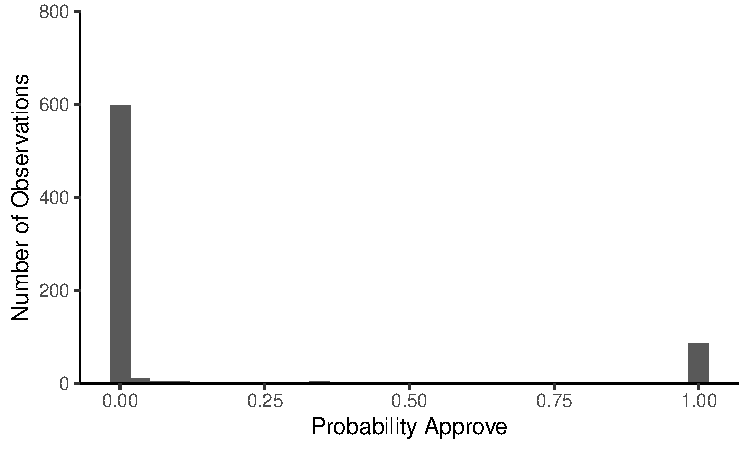
\includegraphics{05.Figures/stance_strength_unique.pdf}
				\begin{minipage}{\textwidth} 
			{\footnotesize Data is sourced from the Department of Transportation regulatory filing regarding the JetBlue-Spirit merger (DOT-OST-2023-0024). ``Probability Approve" is the probability that a comment approves of the merger.} 
		\end{minipage}
	\end{figure}
	
	
\end{appendices}
	
\end{document}